\begingroup
\def\s{\sum\limits_{i=1}^\infty }
\def\tint{\int_{-\pi}^{\pi}}

\chapter{无穷级数}
无穷级数是高等数学的一个重要组成部分;
它是表示函数,研究函数性质,以及进行数值计算的一种工具.
本章先讨论常数项级数,介绍无穷级数的一些基本内容,然后讨论函数项级数,
着重讨论如何将函数展开成幂级数和三角级数的问题.

\section{常数项级数的概念和性质}
人们认识事物在数量方面的特性,往往有一个由近似到精确的过程.
在这种认识过程中,会遇到由有限个数量相加到无穷多个数量相加的问题.

例如计算半径为\(R\)的圆面积\(A\),具体做法如下:
如\cref{figure:无穷级数.用内接正多边形覆盖圆},
作圆的内接正六边形,算出这六边形的面积\(a_1\),它是圆面积\(A\)的一个粗糙的近似值.
为了比较准确地计算出\(A\)的值,
我们以这个正六边形的每一边为底分别作一个顶点在圆周上的等腰三角形,
算出这六个等腰三角形的面积之和\(a_2\).
那么\(a_1+a_2\)(即内接正十二边形的面积)就是\(A\)的一个较好的近似值.
同样地,在这正十二边形的每一边上分别作一个顶点在圆周上的等腰三角形,
算出这十二个等腰三角形的面积之和\(a_3\).
那么\(a_1+a_2+a_3\)(即内接正二十四边形的面积)是\(A\)的一个更好的近似值.
如此继续下去,内接\(3\cdot2^n\)边形的面积就逐步逼近圆面积:\[
	A \approx a_1 + a_2 + \dotsb + a_n.
\]

\begin{figure}[h]
	\centering
	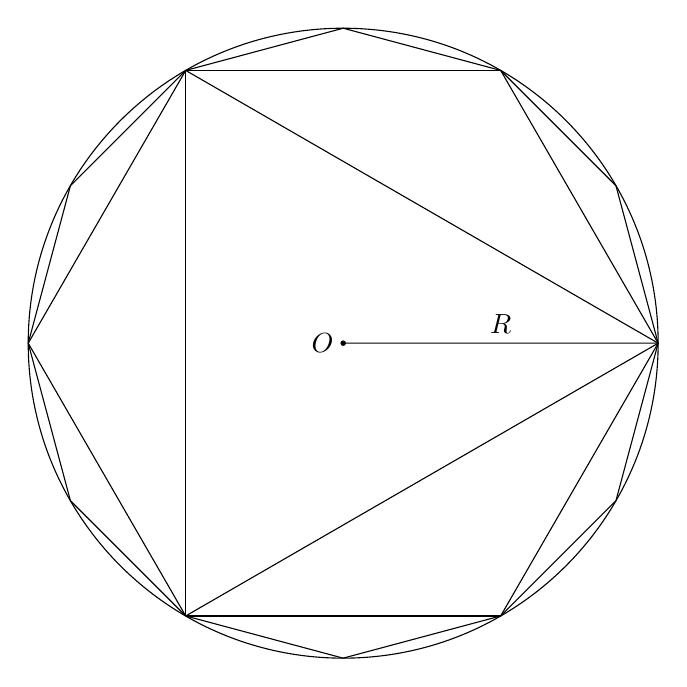
\begin{tikzpicture}
		\pgfmathsetmacro{\radius}{4}
		\def\PlotPolygon#1{
			\foreach \i in {1,...,#1}{
				\draw({\radius*cos(\i*360/#1)},{\radius*sin(\i*360/#1)})
				--({\radius*cos((\i-1)*360/#1)},{\radius*sin((\i-1)*360/#1)});
			}
		}
		\begin{scope}
			\PlotPolygon{3}
			\PlotPolygon{6}
			\PlotPolygon{12}
		\end{scope}
		\draw(0,0)circle(\radius)node[left]{\(O\)}
			--(\radius,0)node[midway,above]{\(R\)};
		\fill(0,0)circle(1pt);

	\end{tikzpicture}
	\caption{用内接正多边形覆盖圆}
	\label{figure:无穷级数.用内接正多边形覆盖圆}
\end{figure}

如果内接正多边形的边数无限增多,即\(n\)无限增大,
则和\(a_1+a_2+\dotsb+a_n\)的极限就是所要求的圆面积\(A\).
这时和式中的项数无限增多,于是出现了无穷多个数量依次相加的数学式子.

\subsection{常数项级数的概念}
\begin{definition}\label{definition:无穷级数.常数项级数的定义}
一般地,给定一个有无穷多项的数列\[
	u_1,u_2,\dotsc,u_n,\dotsc,
\]
则由该数列构成的表达式\[
	u_1+u_2+\dotsb+u_n+\dotsb
\]
叫做\DefineConcept{常数项无穷级数}(infinite series with constant terms),
简称\DefineConcept{常数项级数},
记作\(\sum\limits_{n=1}^\infty u_n\),
即\[
	\sum\limits_{n=1}^\infty u_n
	\defeq
	u_1+u_2+\dotsb+u_n+\dotsb,
\]
其中第\(n\)项\(u_n\)叫做级数的\DefineConcept{一般项}.

作常数项级数的前\(n\)项的和\[
	s_n = u_1+u_2+\dotsb+u_n = \sum\limits_{i=1}^n{u_i}.
\]
我们把\(s_n\)称为级数\(\sum\limits_{n=1}^\infty u_n\)的\DefineConcept{部分和}(partial sum).

如果级数\(\sum\limits_{n=1}^\infty u_n\)的部分和数列\(\{s_n\}\)有极限\(s\),即\[
	\lim\limits_{n\to\infty} s_n = s,
\]
则称“无穷级数\(\sum\limits_{n=1}^\infty u_n\) \DefineConcept{收敛}(converge)”,
这时极限\(s\)叫做这级数的\DefineConcept{和}(sum),并写成\[
	s = u_1+u_2+\dotsb+u_n+\dotsb;
\]
反之,如果\(\{s_n\}\)没有极限,
则称“无穷级数\(\sum\limits_{n=1}^\infty u_n\) \DefineConcept{发散}(diverge)”.

显然,当级数收敛时,其部分和\(s_n\)是级数的和\(s\)的近似值,它们之间的差值\[
	r_n = s - s_n = u_{n+1}+u_{n+2}+\dotsb
\]
叫做“级数\(\sum\limits_{n=1}^\infty u_n\)的\DefineConcept{余项}”.
称这个余项的绝对值\(\abs{r_n}\)为%
“用近似值\(s_n\)代替和\(s\)所产生的\DefineConcept{误差}”.
\end{definition}
从上述定义可知,级数与数列极限有着紧密的联系.给定级数\(\sum\limits_{n=1}^\infty u_n\),
就有部分和数列\(\{s_n = \sum\limits_{i=1}^n u_n\}\);
反之,给定数列\(\{s_n\}\),就有以\(\{s_n\}\)为部分和数列的级数\[
	s_1 + (s_2-s_1) + \dotsb + (s_n-s_{n-1}) + \dotsb
	= s_1 + \sum\limits_{i=2}^\infty (s_i-s_{i-1})
	= \sum\limits_{n=1}^\infty u_n,
\]
其中\(u_1=s_1\),\(u_n=s_n-s_{n-1}\ (n \geq 2)\).
按定义,级数\(\sum\limits_{n=1}^\infty u_n\)与数列\(\{s_n\}\)同时收敛或同时发散,
且在收敛时,有\[
	\sum\limits_{n=1}^\infty u_n = \lim\limits_{n\to\infty} s_n,
\]
即\(\sum\limits_{n=1}^\infty u_n = \lim\limits_{n\to\infty} \sum\limits_{i=1}^n u_n\).

\begin{example}\label{example:无穷级数.等比级数的收敛性}
无穷级数\[
	\sum\limits{n=1} a q^n
	= a+aq+aq^2+\dotsb+aq^n+\dotsb
\]
叫做\DefineConcept{等比级数}或\DefineConcept{几何级数},
其中\(a \neq 0\),\(q\)叫做\DefineConcept{级数的公比}.
试讨论上述等比级数的收敛性.
\begin{solution}
当\(q = 1\)时,则部分和\(s_n=na\),那么\(\lim\limits_{n\to\infty} s_n = \lim\limits_{n\to\infty} na = \infty\),即级数发散.

当\(q \neq 1\),则\[
s_n = \frac{a(1-q^n)}{1-q} = \frac{a}{1-q} - \frac{aq^n}{1-q}.
\]
当\(\abs{q} < 1\)时由于\(\lim\limits_{n\to\infty} q^n=0\),从而\(\lim\limits_{n\to\infty} s_n=\frac{a}{1-q}\),
因此级数收敛,其和为\(\frac{a}{1-q}\).
当\(\abs{q} > 1\)时由于\(\lim\limits_{n\to\infty} q^n=\infty\),从而\(\lim\limits_{n\to\infty} s_n=\infty\),即级数发散.
当\(q = -1\)时,级数变为\(a-a+a-a+\dotsb\),
显然\(s_n\)随着\(n\)为奇数或为偶数而等于\(a\)或等于零,从而\(s_n\)的极限不存在,这是级数也发散.

综上所述,{\color{red}当\(\abs{q} < 1\)时,几何级数收敛;当\(\abs{q} \geq 1\)时,几何级数发散.}
\end{solution}
\end{example}

\begin{example}\label{example:无穷级数.等差级数的收敛性}
试证级数\[
1+2+3+\dotsb+n+\dotsb
\]是发散的.
\begin{proof}
级数的部分和为\[
s_n = 1+2+3+\dotsb+n = \frac{n(n+1)}{2}.
\]显然,\(\lim\limits_{n\to\infty} s_n=\infty\),级数是发散的.
\end{proof}
\end{example}
从上例也可看出:
\begin{proposition}
除非初项\(a_0\)与公差\(d\)都等于\(0\),
否则等差级数\(\sum\limits_{n=0}^\infty(a_0+nd)\)总是发散的.
\end{proposition}

\begin{example}
判定无穷级数\[
\frac{1}{1\cdot2}+\frac{1}{2\cdot3}+\dotsb+\frac{1}{n(n+1)}+\dotsb
\]的收敛性.
\begin{solution}
记\[
	u_n = \frac{1}{n(n+1)} = \frac{1}{n}-\frac{1}{n+1},
\]
因此\begin{align*}
	s_n &= \frac{1}{1\cdot2}+\frac{1}{2\cdot3}+\dotsb+\frac{1}{n(n+1)} \\
	&= \left(1-\frac{1}{2}\right)+\left(\frac{1}{2}-\frac{1}{3}\right)
	+\dotsb+\left(\frac{1}{n}-\frac{1}{n+1}\right) \\
	&= 1-\frac{1}{n+1}.
\end{align*}
从而\[
	\lim\limits_{n\to\infty} s_n = \lim\limits_{n\to\infty} \left(1-\frac{1}{n+1}\right) = 1,
\]
即该级数收敛,它的和为\(1\).
\end{solution}
\end{example}

\subsection{收敛级数的基本性质}
\begin{property}\label{theorem:无穷级数.收敛级数性质1}
如果级数\(\sum\limits_{n=1}^\infty u_n\)收敛于和\(s\),
则级数\(\sum\limits_{n=1}^\infty k u_n\)收敛于和\(ks\).
\begin{proof}
设级数\(\sum\limits_{n=1}^\infty u_n\)
与级数\(\sum\limits_{n=1}^\infty k u_n\)的
部分和分别为\(s_n\)与\(\sigma_n\),
则\[
	\sigma_n
	= k u_1 + k u_2 + \dotsb + k u_n
	= k(u_1 + u_2 + \dotsb + u_n) = k s_n,
\]\[
	\lim\limits_{n\to\infty} \sigma_n
	= \lim\limits_{n\to\infty} k s_n
	= k \lim\limits_{n\to\infty} s_n = ks,
\]
也就是说,级数\(\sum\limits_{n=1}^\infty k u_n\)收敛于\(ks\).

特别地,对于任意发散级数\(\sum\limits_{n=1}^\infty u_n\),
级数\(\sum\limits_{n=1}^\infty 0 \cdot u_n\)的每一项都是零,
故级数\(\sum\limits_{n=1}^\infty 0 \cdot u_n\)收敛于\(0\).
\end{proof}
\end{property}

由关系式\(\sigma_n = k s_n\)知道,
如果\(\{s_n\}\)没有极限且\(k\neq0\),
那么\(\{\sigma_n\}\)也不可能有极限.
因此我们得到如下结论:
{\color{red}级数的每一项同乘一个非零常数后,它的敛散性不会改变.}

\begin{example}
判断\[
\sin\frac{\pi}{6}+\sin\frac{2\pi}{6}+\dotsb+\sin\frac{n\pi}{6}+\dotsb
\]的收敛性.
\begin{solution}
记\(u_n = \sin\frac{n\pi}{6},
v_n = 2\sin\frac{\pi}{12} \cdot u_n\).
因为\[
	v_n = \cos\frac{\pi-2n\pi}{12} - \cos\frac{\pi+2n\pi}{12},
\]\[
	\sigma_n
	= v_1 + v_2 + \dotsb + v_n
	= \cos\frac{\pi}{12} - \cos\frac{(2n+1)\pi}{12},
\]
所以\[
	s_n
	= \left(2\sin\frac{\pi}{12}\right)^{-1} \cdot \sigma_n
	= 1+\frac{\sqrt{3}}{2} - \frac{\sqrt{2}}{\sqrt{3}-1} \cos\frac{(2n+1)\pi}{12}.
\]
可见\(\lim\limits_{n\to\infty} s_n\)不存在,级数发散.
\end{solution}
\end{example}

\begin{property}\label{theorem:无穷级数.收敛级数性质2}
如果级数\(\sum\limits_{n=1}^\infty u_n\)、\(\sum\limits_{n=1}^\infty v_n\)分别收敛于\(s\)、\(\sigma\),
则级数\(\sum\limits_{n=1}^\infty(u_n \pm v_n)\)收敛于\(s \pm \sigma\).
\begin{proof}
设级数\(\sum\limits_{n=1}^\infty u_n\)与级数\(\sum\limits_{n=1}^\infty v_n\)的部分和分别为\(s_n\)与\(\sigma_n\),
则级数\(\sum\limits_{n=1}^\infty(u_n \pm v_n)\)的部分和\begin{align*}
	\tau_n &= (u_1 \pm v_1) + (u_2 \pm v_2) + \dotsb + (u_n + v_n) \\
	&= (u_1 + u_2 + \dotsb + u_n) \pm (v_1 + v_2 + \dotsb + v_n) \\
	&= s_n \pm \sigma_n,
\end{align*}
于是\[
	\lim\limits_{n\to\infty} \tau_n
	= \lim\limits_{n\to\infty} (s_n \pm \sigma_n)
	= s + \sigma.
\]

这就表明级数\(\sum\limits_{n=1}^\infty(u_n \pm v_n)\)收敛于\(s \pm \sigma\).
\end{proof}
\end{property}
\cref{theorem:无穷级数.收敛级数性质2} 也可以说成:
{\color{red}两个收敛级数可以逐项相加、逐项相减.}

\begin{example}
设级数\(\sum\limits_{n=1} u_n\)收敛,\(\sum\limits_{n=1} v_n\)发散.
试证:级数\(\sum\limits_{n=1} (u_n \pm v_n)\)发散.
\begin{proof}
设级数\(\sum\limits_{n=1} u_n\)与\(\sum\limits_{n=1} v_n\)的部分和分别为\(s_n\)和\(\sigma_n\),又设\[
\lim\limits_{n\to\infty} s_n = s.
\]
假设级数\(\sum\limits_{n=1} (u_n \pm v_n)\)收敛,且\[
\lim\limits_{n\to\infty} (s_n \pm \sigma_n) = s+\sigma,
\]那么根据\hyperref[theorem:极限.极限的四则运算法则]{极限的四则运算法则}\[
\lim\limits_{n\to\infty} \pm\sigma_n
= \lim\limits_{n\to\infty} [(s_n \pm \sigma_n) - s_n]
= \lim\limits_{n\to\infty} (s_n \pm \sigma_n) - \lim\limits_{n\to\infty} s_n
= (s + \sigma) - s
= \sigma,
\]也就是说\(\{\pm\sigma_n\}\)(即\(\pm\sum\limits_{n=1} v_n\))收敛,矛盾!
\end{proof}
\end{example}
从上例我们可以看出:
{\color{red}一个收敛级数与一个发散级数相加(或相减)所得级数必定发散.}

另一方面,任给一个发散级数\(\sum\limits_{n=1} u_n\),
级数\(\sum\limits_{n=1} u_n + \sum\limits_{n=1} u_n
= \sum\limits_{n=1} 2 u_n\)也是发散的,
而级数\(\sum\limits_{n=1} u_n - \sum\limits_{n=1} u_n
= 0\)却是收敛的,
于是我们还可以看出:
{\color{red}两个发散级数相加(或相减)所得级数可能收敛也可能发散.}

\begin{example}
已知级数\(\sum\limits_{n=1}^\infty (-1)^{n-1} a_n = 2,
\sum\limits_{n=1}^\infty a_{2n-1} = 5\),
求\(\sum\limits_{n=1}^\infty a_n\).
\begin{solution}
由于\(\sum\limits_{n=1}^\infty [a_n + (-1)^{n-1} a_n]
= 2 \sum\limits_{n=1}^\infty a_{2n-1}\)收敛,
所以\(\sum\limits_{n=1}^\infty a_n\)收敛,且有
\[
\sum\limits_{n=1}^\infty a_n
= 2 \sum\limits_{n=1}^\infty a_{2n-1}
- \sum\limits_{n=1}^\infty (-1)^{n-1} a_n
= 10 - 2 = 8.
\]
\end{solution}
\end{example}

\begin{property}\label{theorem:无穷级数.收敛级数性质3}
在级数中去掉、加上或改变有限项,不会改变级数的收敛性.
\begin{proof}
我们只需证明“在级数的前面部分去掉或加上有限项,不会改变级数的收敛性”,
因为其他情形(即在级数中任意去掉、加上或改变有限项的情形)都可以看成在级数的前面部分先去掉有限项,
然后再加上有限项的结果.

将级数\[
u_1+u_2+\dotsb+u_k+u_{k+1}+\dotsb+u_{k+n}+\dotsb
\]的前\(k\)项去掉,则得级数\[
u_{k+1}+u_{k+2}+\dotsb+u_{k+n}+\dotsb.
\]于是新得到的级数的部分和为\[
\sigma_n = u_{k+1}+u_{k+2}+\dotsb+u_{k+n} = s_{k+n} - s_k,
\]其中\(s_{k+n}\)是原级数的前\(k+n\)项的和.
因为\(s_k\)是常数,所以当\(n\to\infty\)时,
\(\sigma_n\)与\(s_{k+n}\)这两个量,要么同时具有极限,要么同时没有极限.

同理可证在级数的前面加上有限项,不会改变级数的收敛性.
由此可见,在级数中去掉、加上或改变有限项,不会改变级数的收敛性.

另外,我们可以观察到,在收敛级数中去掉、加上或改变有限项,
虽不会改变级数的收敛性,但可能会改变收敛级数的和.
\end{proof}
\end{property}

\begin{property}\label{theorem:无穷级数.收敛级数性质4}
如果级数\(\sum\limits_{n=1}^\infty u_n\)收敛,则对这级数的项任意加括号后所成的级数\[
(u_1+\dotsb+u_{n_1}) + (u_{n_1+1}+\dotsb+u_{n_2}) + \dotsb + (u_{n_{k-1}+1}+\dotsb+u_{n_k}) + \dotsb
\]仍收敛,且其和不变.
\end{property}

应该注意到:
如果加括号后所成的级数收敛,则不能断定去括号后原来的级数也收敛.
例如,级数\[
(1-1)+(1-1)+\dotsb
\]收敛于零,但级数\[
1-1+1-1+\dotsb
\]却是发散的.

根据\cref{theorem:无穷级数.收敛级数性质4} 可得如下推论:{\color{red}如果加括号后所成的级数发散,则原来的级数也发散.}
事实上,倘若原级数收敛,则根据\cref{theorem:无穷级数.收敛级数性质4} 知道,加括号后的级数就应该收敛了.

\begin{property}[级数收敛的必要条件]\label{theorem:无穷级数.收敛级数性质5}
如果级数\(\sum\limits_{n=1}^\infty u_n\)收敛,则它的一般项\(u_n\)满足\[
\lim\limits_{n\to\infty} u_n = 0.
\]
\begin{proof}
设级数\(\sum\limits_{n=1}^\infty u_n\)的部分和为\(s_n\),且\(\lim\limits_{n\to\infty} s_n = s\),则\[
\lim\limits_{n\to\infty} u_n = \lim\limits_{n\to\infty}(s_n - s_{n-1}) = \lim\limits_{n\to\infty} s_n - \lim\limits_{n\to\infty} s_{n-1} = s - s = 0.
\qedhere
\]
\end{proof}
\end{property}

根据\cref{theorem:无穷级数.收敛级数性质5} 可知,如果\(\lim\limits_{n\to\infty} u_n \neq 0\),那么\(\sum\limits_{n=1}^\infty u_n\)一定发散.
例如,级数\[
\frac{1}{2}-\frac{2}{3}+\frac{3}{4}-\dotsb+(-1)^{n-1}\frac{n}{n+1}+\dotsb,
\]它的一般项\(u_n = (-1)^{n-1} \frac{n}{n+1}\)当\(n\to\infty\)时不趋于零,因此该级数是发散的.

值得注意的是,级数的一般项趋于零并不是级数收敛的充分条件.
有些级数虽然一般项趋于零,但仍然是发散的.
\begin{example}\label{example:无穷级数.调和级数的收敛性}
试证:调和级数\[
\sum\limits_{n=1}^\infty u_n = 1+\frac{1}{2}+\frac{1}{3}+\dotsb+\frac{1}{n}+\dotsb
\]是发散的.
\begin{proof}
虽然调和级数的一般项\(\lim\limits_{n\to\infty} u_n = \lim\limits_{n\to\infty} 1/n = 0\),但是它是发散的.
现在我们用反证法证明.

假设级数\(\sum\limits_{n=1}^\infty u_n\)收敛.设级数的部分和为\(s_n\),且\(\lim\limits_{n\to\infty} s_n = s\).
显然,对级数\(\sum\limits_{n=1}^\infty u_n\)的部分和\(s_{2n}\)也有\(\lim\limits_{n\to\infty} s_{2n} = s\).
于是\[
\lim\limits_{n\to\infty} {s_{2n}-s_n} = \lim\limits_{n\to\infty} s_{2n} - \lim\limits_{n\to\infty} s_n = s - s = 0.
\]但另一方面\[
s_{2n} - s_n = \frac{1}{n+1}+\frac{1}{n+2}+\dotsb+\frac{1}{2n}
> \underbrace{\frac{1}{2n}+\frac{1}{2n}+\dotsb+\frac{1}{2n}}_{n\text{项}}
= \frac{1}{2},
\]\[
\lim\limits_{n\to\infty} {s_{2n}-s_n} \neq 0,
\]与假设矛盾,说明级数\(\sum\limits_{n=1}^\infty u_n\)必定发散.
\end{proof}
\end{example}

\subsection{柯西审敛原理}
\begin{theorem}[柯西审敛原理]\label{theorem:无穷级数.级数的柯西审敛原理}
级数\(\sum\limits_{n=1}^\infty u_n\)收敛的充要条件为:
对于任意给定的正数\(\epsilon\),总存在正整数\(N\),
使得当\(n>N\)时,对于任意的正整数\(p\),都有\[
\abs{ \sum\limits_{i=1}^p u_{n+i} }
= \abs{u_{n+1}+u_{n+2}+\dotsb+u_{n+p}}
< \epsilon
\]成立.
\begin{proof}
设级数\(\sum\limits_{n=1}^\infty u_n\)的部分和为\(s_n\),因为\[
\abs{u_{n+1}+u_{n+2}+\dotsb+u_{n+p}} = \abs{s_{n+p}-s_n},
\]所以由\hyperref[theorem:极限.数列的柯西极限存在准则]{柯西极限存在准则}可得本定理结论.
\end{proof}
\end{theorem}

\begin{example}
试求级数\(\s \frac{1}{n^2}\)的收敛性.
\begin{solution}
因为对任意正整数\(p\),\begin{align*}
&\abs{u_{n+1}+u_{n+2}+\dotsb+u_{n+p}} \\
&=\frac{1}{(n+1)^2}+\frac{1}{(n+2)^2}+\dotsb+\frac{1}{(n+p)^2} \\
&<\frac{1}{n(n+1)}+\frac{1}{(n+1)(n+2)}+\dotsb+\frac{1}{(n+p-1)(n+p)} \\
&=\left(\frac{1}{n}-\frac{1}{n+1}\right)+\left(\frac{1}{n+1}-\frac{1}{n+2}\right)+\dotsb+\left(\frac{1}{n+p-1}-\frac{1}{n+p}\right) \\
&=\frac{1}{n}-\frac{1}{n+p} < \frac{1}{n},
\end{align*}
所以对于\(\forall \epsilon > 0\),取正整数\(N \geq \frac{1}{\epsilon}\),则当\(n > N\)时,对任何正整数\(p\),都有\[
\abs{u_{n+1}+u_{n+2}+\dotsb+u_{n+p}}
< \frac{1}{n}
< \frac{1}{N}
\leq \epsilon
\]成立.
按柯西审敛原理,级数\(\s \frac{1}{n^2}\)收敛.
\end{solution}
\end{example}

\section{常数项级数的审敛法}
\subsection{正项级数及其审敛法}
\subsubsection{正项级数的概念及其收敛条件}
一般的常数项级数,它的各项可以是正数、负数或零.
现在我们先讨论各项都是正数或零的级数,这种级数称为\DefineConcept{正项级数}.
这种级数特别重要,以后将看到许多级数的收敛性问题可归结为正项级数的收敛性问题.

\begin{theorem}\label{theorem:无穷级数.正项级数收敛的充要条件}
%@see: 《高等数学(第六版 下册)》 P256. 定理1
%@see: 《数学分析教程 (第三版 下册)》 P163. 定理14.2.1
正项级数\(\sum\limits_{n=1}^\infty u_n\)收敛的充要条件是:
它的部分和数列\(\{s_n\}\)有界.
\begin{proof}
显然,数列\(\{s_n\}\)是一个单调增加数列.
如果数列\(\{s_n\}\)有界,
那么根据\hyperref[theorem:极限.数列的单调有界定理]{单调有界定理},
数列\(\{s_n\}\)收敛,
也就是说,级数\(\sum\limits_{n=1}^\infty u_n\)收敛.

反之,如果正项级数\(\sum\limits_{n=1}^\infty u_n\)收敛于和\(s\),
即\(\lim\limits_{n\to\infty} s_n = s\),
根据\hyperref[theorem:极限.收敛数列的有界性]{收敛数列的有界性}可知,
数列\(\{s_n\}\)有界.
\end{proof}
\end{theorem}

我们可以写出\cref{theorem:无穷级数.正项级数收敛的充要条件} 的逆否命题.
\begin{proposition}
正项级数\(\sum\limits_{n=1}^\infty u_n\)发散的充要条件是它的部分和数列无界.
\end{proposition}

\begin{example}
%@see: 《数学分析教程 (第三版 下册)》 P163. 例1
设正项级数\(\sum\limits_{n=1}^\infty a_n\)的部分和是\(s_n\),证明:\[
	\sum\limits_{n=1}^\infty \frac{a_n}{s_n^2} < +\infty.
\]
\begin{proof}
显然\(\sum\limits_{n=1}^\infty \frac{a_n}{s_n^2}\)是正项级数.
由于对于任意正整数\(N\),有\begin{align*}
	\sum_{n=2}^N \frac{a_n}{s_n^2}
	&= \sum_{n=2}^N \frac{s_n-s_{n-1}}{s_n^2}
	\leq \sum_{n=2}^N \frac{s_n-s_{n-1}}{s_{n-1} s_n} \\
	&= \sum_{n=2}^N \left(
			\frac{1}{s_{n-1}} - \frac{1}{s_n}
		\right)
	= \frac{1}{s_1} - \frac{1}{s_N}
	< \frac{1}{a_1},
\end{align*}
也就是说\(\sum\limits_{n=1}^\infty \frac{a_n}{s_n^2}\)的部分和有界,
所以根据\cref{theorem:无穷级数.正项级数收敛的充要条件},该级数收敛.
\end{proof}
\end{example}

\begin{example}
设正项级数\(\sum\limits_{n=1}^\infty a_n\)的部分和是\(s_n\),
证明:对于任意\(k>1\),有\[
	\sum_{n=1}^\infty \frac{a_n}{s_n^k} < +\infty.
\]
%TODO
\end{example}

\subsubsection{比较审敛法}
\begin{theorem}[比较审敛法]\label{theorem:无穷级数.正项级数的比较审敛法}
设\(\sum\limits_{n=1}^\infty u_n\)和\(\sum\limits_{n=1}^\infty v_n\)都是正项级数,且\[
u_n \leq v_n
\quad(n=1,2,\dotsc).
\]
若级数\(\sum\limits_{n=1}^\infty v_n\)收敛,则级数\(\sum\limits_{n=1}^\infty u_n\)收敛;
反之,若级数\(\sum\limits_{n=1}^\infty u_n\)发散,则级数\(\sum\limits_{n=1}^\infty v_n\)发散.
\begin{proof}
设级数\(\sum\limits_{n=1}^\infty v_n\)收敛于和\(\sigma\),则级数\(\sum\limits_{n=1}^\infty u_n\)的部分和\[
s_n = u_1 + u_2 + \dotsb u_n
\leq
v_1 + v_2 + \dotsb + v_n \leq \sigma
\quad(n=1,2,\dotsc),
\]
即部分和数列\(\{s_n\}\)有界,
由\cref{theorem:无穷级数.正项级数收敛的充要条件} 知级数\(\sum\limits_{n=1}^\infty u_n\)收敛.
\end{proof}
\end{theorem}

\begin{example}
\def\s{\sum\limits_{n=1}^\infty }
判断级数\(\s \frac{1}{1+a^n}\ (a>0)\)的收敛性.
\begin{solution}
显然有\[
\frac{1}{1+a^n} < \frac{1}{a^n}.
\]根据比较审敛法,如果级数\(\s \frac{1}{a^n}\)收敛,那么级数\(\s \frac{1}{1+a^n}\)收敛;
而等比级数\(\s \frac{1}{a^n}\)当且仅当其公比\(\abs{\frac{1}{a}} < 1\),即\(a > 1\)时收敛;
故当\(a > 1\)时,级数\(\s \frac{1}{1+a^n}\)收敛.

当\(0 < a \leq 1\)时,\(0 < a^n \leq 1\),\(1 < 1 + a^n \leq 2\),\[
\frac{1}{1+a^n} \geq \frac{1}{2},
\]而等差级数\(\s \frac{1}{2}\)发散,故级数\(\s \frac{1}{1+a^n}\)发散.
\end{solution}
\end{example}

注意到级数的每一项同乘不为零的常数\(k\)以及去掉级数前面部分的有限项不会影响级数的收敛性,我们可得如下推论:
\begin{corollary}\label{theorem:无穷级数.正项级数的比较审敛法的推论}
设\(\sum\limits_{n=1}^\infty u_n\)和\(\sum\limits_{n=1}^\infty v_n\)都是正项级数.
如果级数\(\sum\limits_{n=1}^\infty v_n\)收敛,且存在正整数\(N\),使当\(n \geq N\)时有\(u_n \leq k v_n\ (k > 0)\)成立,则级数\(\sum\limits_{n=1}^\infty u_n\)收敛;
如果级数\(\sum\limits_{n=1}^\infty v_n\)发散,且存在正整数\(N\),使当\(n \geq N\)时有\(u_n \geq k v_n\ (k > 0)\)成立,则级数\(\sum\limits_{n=1}^\infty u_n\)发散.
\end{corollary}

\begin{example}
试证:级数\(\sum\limits_{n=1}^\infty \frac{1}{\sqrt{n(n+1)}}\)是发散的.
\begin{proof}
因为\(n(n+1) < (n+1)^2\),所以\(\frac{1}{\sqrt{n(n+1)}} > \frac{1}{n+1}\),而级数\(\sum\limits_{n=1}^\infty \frac{1}{n+1}\)是发散的,根据比较审敛法可知级数\(\sum\limits_{n=1}^\infty \frac{1}{\sqrt{n(n+1)}}\)是发散的.
\end{proof}
\end{example}

\subsubsection{p级数}
\begin{example}\label{example:无穷级数.p级数的收敛性}
讨论p级数\[
1+\frac{1}{2^p}+\frac{1}{3^p}+\dotsb+\frac{1}{n^p}+\dotsb
\]的收敛性,其中常数\(p>0\).
\begin{solution}
当\(p \leq 1\)时,p级数各项均不小于调和级数对应项,即\(\frac{1}{n^p} \geq \frac{1}{n}\),但调和级数发散,故根据\cref{theorem:无穷级数.正项级数的比较审敛法} 可知,当\(p \leq 1\)时p级数发散.

当\(p > 1\)时,因为\(k-1 \leq x \leq k \implies \frac{1}{k} \leq \frac{1}{x} \implies \frac{1}{k^p} \leq \frac{1}{x^p}\),所以\[
\frac{1}{k^p}
= \int_{k-1}^k \frac{1}{k^p} \dd{x}
\leq \int_{k-1}^k \frac{1}{x^p} \dd{x}
\quad(k=2,3,\dotsc),
\]
从而级数的部分和
\begin{align*}
s_n &= 1 + \sum\limits_{k=2}^n{\frac{1}{k^p}}
\leq 1 + \sum\limits_{k=2}^n{ \int_{k-1}^k{\frac{1}{x^p}\dd{x}} }
= 1 + \int_1^n{\frac{1}{x^p}\dd{x}} \\
&= 1 + \frac{1}{p-1}\left(1-\frac{1}{n^{p-1}}\right)
< 1 + \frac{1}{p-1}
\quad(n=2,3,\dotsc),
\end{align*}
这表明数列\(\{s_n\}\)有界,因此p级数收敛.

综上所述,{\color{red} p级数\(\sum\limits_{n=1}^\infty \frac{1}{n^p}\)当\(p > 1\)时收敛,当\(p \leq 1\)时发散.}
\end{solution}
\end{example}
可以发现,p级数与\hyperref[example:定积分.p积分]{p积分}具有高度相似性.

\begin{example}
设正项级数\(\sum\limits_{n=1}^\infty a_n\)发散,证明:级数\(\sum\limits_{n=1}^\infty \frac{a_n}{n^3+a_n^2}\)收敛.
\begin{proof}
由基本不等式 \labelcref{theorem:不等式.基本不等式1} 可知
\(n^3+a_n^2\geq2\sqrt{n^3 a_n^2}=2n^{3/2}a_n\),
那么\(\frac{a_n}{n^3+a_n^2}\leq\frac{a_n}{2n^{3/2}a_n}=\frac{1}{2n^{3/2}}\).
由\cref{example:无穷级数.p级数的收敛性}
我们知道\(p=\frac{3}{2}>1\)时,p级数收敛;
那么根据\hyperref[theorem:无穷级数.正项级数的比较审敛法]{比较审敛法}可知
级数\(\sum\limits_{n=1}^\infty \frac{a_n}{n^3+a_n^2}\)收敛.
\end{proof}
\end{example}

\subsubsection{比较审敛法的极限形式}
\begin{theorem}[比较审敛法的极限形式]\label{theorem:无穷级数.正项级数的比较审敛法的极限形式}
设\(\sum\limits_{n=1}^\infty u_n\)和\(\sum\limits_{n=1}^\infty v_n\)都是正项级数,记\[
l = \lim\limits_{n\to\infty} \frac{u_n}{v_n}.
\]\begin{enumerate}
\item 如果\(l\in[0,+\infty)\),且级数\(\sum\limits_{n=1}^\infty v_n\)收敛,则级数\(\sum\limits_{n=1}^\infty u_n\)收敛;
\item 如果\(l\in(0,+\infty]\),且级数\(\sum\limits_{n=1}^\infty v_n\)发散,则级数\(\sum\limits_{n=1}^\infty u_n\)发散.
\end{enumerate}
\begin{proof}
如果\(\lim\limits_{n\to\infty} {\frac{u_n}{v_n}}=l\in[0,+\infty)\),
那么由极限定义可知,对\(\epsilon=1\),
\(\exists N\in\mathbb{N}\),
对于\(\forall n\in\mathbb{N}\),
只要\(n>N\),就有\[
	\frac{u_n}{v_n} < l+1,
\]
即\(u_n < (l+1) v_n\).
而级数\(\sum\limits_{n=1}^\infty v_n\)收敛,
根据\cref{theorem:无穷级数.正项级数的比较审敛法的推论} 可知,
级数\(\sum\limits_{n=1}^\infty u_n\)收敛.

如果\(\lim\limits_{n\to\infty} {\frac{u_n}{v_n}}=l\in(0,+\infty]\),
那么极限\(\lim\limits_{n\to\infty} \frac{v_n}{u_n}\)存在.
如果级数\(\sum\limits_{n=1}^\infty u_n\)收敛,则由上可知必有级数\(\sum\limits_{n=1}^\infty v_n\)收敛,
但已知级数\(s v_i\)发散,因此级数\(\sum\limits_{n=1}^\infty u_n\)不可能收敛,即级数\(\sum\limits_{n=1}^\infty u_n\)发散.
\end{proof}
\end{theorem}

极限形式的比较审敛法,在两个正项级数的一般项均趋于零的情况下,
其实是比较它们的一般项作为无穷小量的阶.
定理表明,当\(n \to \infty\)时,
如果\(u_n\)是与\(v_n\)同阶或是比\(v_n\)高阶的无穷小,
而级数\(\sum\limits_{n=1}^\infty v_n\)收敛,则级数\(\sum\limits_{n=1}^\infty u_n\)收敛;
如果\(u_n\)是与\(v_n\)同阶或是比\(v_n\)低阶的无穷小,
而级数\(\sum\limits_{n=1}^\infty v_n\)发散,则级数\(\sum\limits_{n=1}^\infty u_n\)发散.

\begin{example}
判断级数\(\sum\limits_{n=1}^\infty \sin\frac{1}{n}\)的收敛性.
\begin{solution}
因为\[
\lim\limits_{n\to\infty} \frac{\sin(1/n)}{1/n} = 1 > 0,
\]而级数\(\sum\limits_{n=1}^\infty \frac{1}{n}\)发散,可知级数\(\sum\limits_{n=1}^\infty \sin\frac{1}{n}\)发散.
\end{solution}
\end{example}

\begin{example}
判断级数\[
1 + \frac{1}{3} + \frac{1}{5} + \dotsb + \frac{1}{2n-1} + \dotsb
\]的收敛性.
\begin{solution}
记\(u_n = \frac{1}{2n-1}\),取\(v_n = \frac{1}{n}\).因为\[
\lim\limits_{n\to\infty} \frac{u_n}{v_n} = \lim\limits_{n\to\infty} \frac{n}{2n-1} = \lim\limits_{n\to\infty} \frac{1}{2-1/n} = \frac{1}{2} > 0,
\]而级数\(\sum\limits_{n=1}^\infty \frac{1}{n}\)发散,所以级数\(\sum\limits_{n=1}^\infty \frac{1}{2n-1}\)发散.
\end{solution}
\end{example}

\begin{example}
判断级数\[
1 + \frac{1+2}{1+2^2} + \frac{1+3}{1+3^2} + \dotsb + \frac{1+n}{1+n^2} + \dotsb
\]的收敛性.
\begin{solution}
记\(u_n = \frac{1+n}{1+n^2}\),取\(v_n = \frac{1}{1+n}\).
因为\[
\lim\limits_{n\to\infty} \frac{u_n}{v_n}
= \lim\limits_{n\to\infty} \frac{(1+n)^2}{1+n^2}
= \lim\limits_{n\to\infty} \frac{n^2 + 2n + 1}{n^2 + 1}
= 1 > 0,
\]而\(\sum\limits_{n=1}^\infty v_n\)发散,所以级数\(\sum\limits_{n=1}^\infty \frac{1+n}{1+n^2}\)发散.
\end{solution}
\end{example}

\begin{example}
判断级数\[
\frac{1}{2\cdot5} + \frac{1}{3\cdot6} + \dotsb + \frac{1}{(n+1)(n+4)} + \dotsb
\]的收敛性.
\begin{solution}
记\(u_n = \frac{1}{(n+1)(n+4)}\),取\(v_n = \frac{1}{n^2}\).
因为\[
\lim\limits_{n\to\infty} \frac{u_n}{v_n} = \lim\limits_{n\to\infty} \frac{n^2}{(n+1)(n+4)} = 1,
\]而级数\(\sum\limits_{n=1}^\infty v_n\)收敛,所以级数\(\sum\limits_{n=1}^\infty \frac{1+n}{1+n^2}\)收敛.
\end{solution}
\end{example}

\begin{example}
\newcommand\sinfrac[1][]{\sin\frac{\pi}{2^{#1}}}
判断级数\[
\sinfrac + \sinfrac[2] + \sinfrac[3] + \dotsb + \sinfrac[n] + \dotsb
\]的收敛性.
\begin{solution}
记\(u_n = \sin\frac{\pi}{2^n}\),取\(v_n = \frac{\pi}{2^n}\).
因为\[
\lim\limits_{n\to\infty} \frac{u_n}{v_n}
= \lim\limits_{n\to\infty} \frac{\sin(\pi/2^n)}{\pi/2^n} = 1,
\]而级数\(\sum\limits_{n=1}^\infty v_n\)收敛,所以级数\(\sum\limits_{n=1}^\infty \sin\frac{\pi}{2^n}\)收敛.
\end{solution}
\end{example}

\subsubsection{比值审敛法}
用比较审敛法审敛时,需要适当地选取一个已知其收敛性的级数\(\sum\limits_{n=1}^\infty v_n\)作为比较的基准.最常选用作为基准级数的是等比级数和p级数.

将所给正项级数与等比级数比较,我们能得到在实用上很方便的比值审敛法和根值审敛法.
\begin{theorem}[比值审敛法,达朗贝尔判别法]\label{theorem:无穷级数.正项级数的比值审敛法}
设\(\sum\limits_{n=1}^\infty u_n\)为正项级数,如果\[
\lim\limits_{n\to\infty} \frac{u_{n+1}}{u_n}=\rho,
\]则当\(\rho<1\)时,级数收敛;
当\(\rho>1\)时或当\(\lim\limits_{n\to\infty} \frac{u_{n+1}}{u_n}=\infty\)时,级数发散;
当\(\rho=1\)时,级数可能收敛也可能发散.
\begin{proof}
当\(\rho<1\).取一个适当小的正数\(\epsilon\),使得\(\rho+\epsilon=r<1\),根据极限定义,存在正整数\(m\),当\(n \geq m\)时有不等式\[
\frac{u_{n+1}}{u_n} < \rho + \epsilon = r.
\]因此\[
u_{m+1} < r u_m,
u_{m+2} < r u_{m+1} < r^2 u_m,
\dotsc,
u_{m+k} < r^k u_m,
\dotsc.
\]而因为公比\(r<1\),故等比级数\(\sum\limits_{k=1}^\infty r^k u_m\)收敛,根据\cref{theorem:无穷级数.正项级数的比较审敛法的推论} 可知,级数\(\sum\limits_{n=1}^\infty u_n\)收敛.

当\(\rho>1\).取一个适当小的正数\(\epsilon\),使得\(\rho-\epsilon>1\).
根据极限定义,当\(n \geq m\)时有不等式\[
\frac{u_{n+1}}{u_n} > \rho-\epsilon > 1,
\]也就是\(u_{n+1}>u_n\).所以当\(n \geq m\)时,级数的一般项\(u_n\)是逐渐增大的,从而\[
\lim\limits_{n\to\infty} u_n \neq 0.
\]根据\cref{theorem:无穷级数.收敛级数性质5} (即级数收敛的必要条件)可知,级数\(\sum\limits_{n=1}^\infty u_n\)发散.

类似地,可以证明当\(\lim\limits_{n\to\infty} \frac{u_{n+1}}{u_n} = \infty\)时,级数\(\sum\limits_{n=1}^\infty u_n\)发散.

当\(\rho = 1\)时,级数可能收敛也可能发散.例如p级数不论\(p\)为何值都有\[
\lim\limits_{n\to\infty} \frac{u_{n+1}}{u_n} = \lim\limits_{n\to\infty} \frac{1/(n+1)^p}{1/n^p} = 1.
\]但我们知道,当\(p>1\)时p级数收敛,当\(p\leq1\)时p级数发散,因此只根据\(\rho=1\)不能判定级数的收敛性.
\end{proof}
\end{theorem}

\begin{example}\label{example:无穷级数.常数e的级数表示}
证明级数\[
1+\frac{1}{1}+\frac{1}{1\cdot2}+\frac{1}{1\cdot2\cdot3}+\dotsb+\frac{1}{(n-1)!}+\dotsb
\]是收敛的,并估计以级数的部分和\(s_n\)近似代替和\(s\)所产生的误差.
\begin{solution}
因为\[
\lim\limits_{n\to\infty} \frac{u_{n+1}}{u_n} = \lim\limits_{n\to\infty} \frac{(n-1)!}{n!} = \lim\limits_{n\to\infty} \frac{1}{n} = 0 < 1,
\]根据比值审敛法可知,该级数收敛.

以该级数的部分和近似代替和\(s\)所产生的的误差为\[
\begin{split}
\abs{r_n} &= \frac{1}{n!} + \frac{1}{(n+1)!} + \frac{1}{(n+2)!} + \dotsb \\
&= \frac{1}{n!} \left[ 1 + \frac{1}{n+1} + \frac{1}{(n+1)(n+2)} + \dotsb \right] \\
&< \frac{1}{n!} \left( 1 + \frac{1}{n} + \frac{1}{n^2} + \dotsb \right) \\
&= \frac{1}{n!} \frac{1}{1-1/n}
= \frac{1}{(n-1)\cdot(n-1)!}.
\end{split}
\]
\end{solution}
\end{example}

\begin{example}
\newcommand\myfrac[1][]{
\def\a{\ifx\relax#1\relax1\else#1\fi}
\frac{3^{#1}}{\a\cdot2^{#1}}
}
判断级数\[
\myfrac + \myfrac[2] + \myfrac[3] + \dotsb + \myfrac[n] + \dotsb
\]的收敛性.
\begin{solution}
记\(u_n = \myfrac[n]\).因为\[
\lim\limits_{n\to\infty} \frac{u_{n+1}}{u_n}
= \lim\limits_{n\to\infty} \frac{3}{2}\cdot\frac{n}{n+1}
= \frac{3}{2} > 1,
\]所以级数发散.
\end{solution}
\end{example}

\begin{example}
\def\s{\sum\limits_{n=1}^\infty }
判断级数\(\s \frac{n^2}{3^n}\)的收敛性.
\begin{solution}
记\(u_n = \frac{n^2}{3^n}\).因为\[
\lim\limits_{n\to\infty} \frac{u_{n+1}}{u_n}
= \lim\limits_{n\to\infty} \frac{1}{3} \cdot \frac{(n+1)^2}{n^2}
= \frac{1}{3} < 1,
\]所以级数收敛.
\end{solution}
\end{example}

\begin{example}
判断级数\(\sum\limits_{n=1}^\infty \frac{2^n \cdot n!}{n^n}\)的收敛性.
\begin{solution}
记\(u_n = \frac{2^n \cdot n!}{n^n}\).
因为\begin{align*}
	\lim\limits_{n\to\infty} \frac{u_{n+1}}{u_n}
	&= \lim\limits_{n\to\infty} 2(n+1) \cdot \frac{n^n}{(n+1)^{n+1}} \\
	&= 2 \cdot \lim\limits_{n\to\infty} \frac{n^n}{(n+1)^n}
	= 2 \cdot \lim\limits_{n\to\infty} \frac{1}{\left(1+\frac{1}{n}\right)^n} \\
	&= 2 \left[ \lim\limits_{n\to\infty} \left(1+\frac{1}{n}\right)^n \right]^{-1}
	= \frac{2}{e} < 1,
\end{align*}
所以级数收敛.
\end{solution}
\end{example}

\begin{example}
判断级数\(\sum\limits_{n=1}^\infty n \tan\frac{\pi}{2^{n+1}}\)的收敛性.
\begin{solution}
记\(u_n = n \tan\frac{\pi}{2^{n+1}}\).我们有\[
	\frac{u_{n+1}}{u_n}
	= \frac{n+1}{n} \frac{\tan(\frac{1}{2}\frac{\pi}{2^{n+1}})}{\tan\frac{\pi}{2^{n+1}}}.
\]
根据二倍角公式\[
	\tan2\theta = \frac{2\tan\theta}{1-\tan^2\theta},
	\qquad
	\frac{\tan\theta}{\tan2\theta} = \frac{1-\tan^2\theta}{2},
\]
有\[
	\frac{\tan(\frac{1}{2}\frac{\pi}{2^{n+1}})}{\tan\frac{\pi}{2^{n+1}}}
	= \frac{1}{2} \left(
		1-\tan^2\frac{\pi}{2^{n+2}}
	\right).
\]
于是\begin{align*}
	\lim\limits_{n\to\infty} \frac{u_{n+1}}{u_n}
	&= \lim\limits_{n\to\infty} \frac{n+1}{n} \frac{1}{2} \left(
		1-\tan^2\frac{\pi}{2^{n+2}}
	\right) \\
	&= \frac{1}{2} \cdot \lim\limits_{n\to\infty} \frac{n+1}{n} \cdot \left(
		1 - \lim\limits_{n\to\infty} \tan^2\frac{\pi}{2^{n+2}}
	\right) \\
	&= \frac{1}{2} \cdot 1 \cdot (1 - 0) = \frac{1}{2} < 1.
\end{align*}
所以级数收敛.
\end{solution}
\end{example}

\subsubsection{比值审敛法的上、下极限形式}
\begin{corollary}[比值审敛法的上、下极限形式]\label{theorem:无穷级数.正项级数的比值审敛法的上下极限形式}
\def\orho{\overline{\rho}}
\def\urho{\underline{\rho}}
设\(\sum\limits_{n=1}^\infty u_n\)为正项级数,记\[
\orho \equiv \varlimsup\limits_{n\to\infty} \frac{a_{n+1}}{a_n},
\qquad
\urho \equiv \varliminf\limits_{n\to\infty} \frac{a_{n+1}}{a_n}.
\]如果\[
\orho < 1,
\]则级数\(\sum\limits_{n=1}^\infty u_n\)收敛;如果\[
\urho > 1,
\]则级数\(\sum\limits_{n=1}^\infty u_n\)发散;如果\[
\orho \geq 1
\quad\lor\quad
\urho \leq 1,
\]则级数可能收敛也可能发散.
\end{corollary}

\subsubsection{根值审敛法}
\begin{theorem}[根值审敛法,柯西判别法]\label{theorem:无穷级数.正项级数的根值审敛法}
设\(\sum\limits_{n=1}^\infty u_n\)为正项级数,如果\[
\lim\limits_{n\to\infty} \sqrt[n]{u_n}=\rho,
\]则当\(\rho<1\)时,级数收敛;
当\(\rho>1\)时或当\(\lim\limits_{n\to\infty} \sqrt[n]{u_n}=+\infty\)时,级数发散;
当\(\rho=1\)时,级数可能收敛也可能发散.
\end{theorem}
在根值审敛法中可以把\(\lim\limits_{n\to\infty}\)替换为\(\varlimsup\limits_{n\to\infty}\).

\begin{example}
\def\s{\sum\limits_{n=1}^\infty }
判定级数\(\s \frac{2+(-1)^n}{2^n}\)的收敛性.
\begin{proof}
记\[
u_n = \frac{2+(-1)^n}{2^n},
\]显然有\[
\lim\limits_{n\to\infty} \sqrt[n]{u_n}
= \lim\limits_{n\to\infty} \frac{1}{2} \sqrt[n]{2+(-1)^n}
= \lim\limits_{n\to\infty} \frac{1}{2} \exp{\frac{1}{n} \ln[2+(-1)^n]},
\]因为\(\ln[2+(-1)^n] \in \{ 0, \ln3 \}\)有界,故\(\lim\limits_{n\to\infty} \frac{1}{n} \ln[2+(-1)^n] = 0\),从而\[
\lim\limits_{n\to\infty} \sqrt[n]{u_n} = \frac{1}{2} < 1.
\]根据根值审敛法可知,级数\(\sum\limits_{n=1}^\infty u_n\)收敛.
\end{proof}
\end{example}

\subsubsection{极限审敛法}
将所给正项级数与p级数作比较,可得在实用上较方便的极限审敛法.
\begin{theorem}[极限审敛法]\label{theorem:无穷级数.正项级数的极限审敛法}
设\(\sum\limits_{n=1}^\infty u_n\)为正项级数.
\begin{enumerate}
\item 当\(\lim\limits_{n\to\infty} n^p u_n = l\in[0,+\infty)\),且\(p>1\)时,级数\(\sum\limits_{n=1}^\infty u_n\)收敛;
\item 当\(\lim\limits_{n\to\infty} n^p u_n = l\in(0,+\infty]\),且\(p\leq1\)时,级数\(\sum\limits_{n=1}^\infty u_n\)发散.
\end{enumerate}
\end{theorem}

\begin{example}
\def\s{\sum\limits_{n=1}^\infty }
判定级数\(\s \ln(1+\frac{1}{n^2})\)的收敛性.
\begin{solution}
因\(\ln(1+\frac{1}{n^2}) \sim \frac{1}{n^2}\ (n\to\infty)\),故\[
\lim\limits_{n\to\infty} n^2 u_n = \lim\limits_{n\to\infty} n^2 \ln(1+\frac{1}{n^2})
= \lim\limits_{n\to\infty} n^2 \cdot \frac{1}{n^2} = 1,
\]根据极限审敛法可知,所给级数收敛.
\end{solution}
\end{example}

\begin{example}
\def\s{\sum\limits_{n=1}^\infty }
判定级数\(\s \sqrt{n+1} \left(1-\cos\frac{\pi}{n}\right)\)的收敛性.
\begin{solution}
因为\(1 - \cos x \sim \frac{1}{2} x^2\ (x\to0)\),故\[
\lim\limits_{n\to\infty} n^{3/2} \sqrt{n+1} \cdot \left(1-\cos\frac{\pi}{n}\right)
= \lim\limits_{n\to\infty} n^2 \sqrt{\frac{n+1}{n}} \cdot \frac{1}{2} \left(\frac{\pi}{n}\right)^2
= \frac{1}{2} \pi^2,
\]根据极限审敛法可知,所给级数收敛.
\end{solution}
\end{example}

\subsubsection{积分审敛法}
\begin{theorem}[积分审敛法]\label{theorem:无穷级数.积分审敛法}
设\(\sum\limits_{n=1}^\infty u_n\)为正项级数,又设非负函数\(f\)在\([1,+\infty)\)上单调递减,且\[
u_n = f(n)
\quad(n=1,2,\dotsc).
\]那么级数\(\sum\limits_{n=1}^\infty u_n\)收敛的充要条件是:反常积分\(\int_1^{+\infty} f(x) \dd{x}\)收敛.
\end{theorem}

\subsubsection{比值审敛法与根值审敛法之间的联系}
\begin{theorem}
对于正项数列\(\sum\limits_{n=1}^\infty u_n\),总有\[
\varliminf\limits_{n\to\infty} \frac{u_{n+1}}{u_n}
\leq
\varliminf\limits_{n\to\infty} \sqrt[n]{u_n}
\leq
\varlimsup\limits_{n\to\infty} \sqrt[n]{u_n}
\leq
\varlimsup\limits_{n\to\infty} \frac{u_{n+1}}{u_n}
\]成立.
\end{theorem}

\subsection{交错级数及其审敛法}
所谓\DefineConcept{交错级数}(alternating series)是这样的级数,
它的各项是正负交错的,从而可以写成下面的形式:\[
u_1 - u_2 + u_3 - u_4 + \dotsb,
\]或\[
-u_1 + u_2 - u_3 + u_4 - \dotsb,
\]其中\(u_1,u_2,\dotsc\)都是正数.

\begin{theorem}[莱布尼茨定理]\label{theorem:无穷级数.莱布尼茨定理}
如果交错级数\(\sum\limits_{n=1}^\infty (-1)^{n-1} u_n\ (u_n>0)\)满足条件:
\begin{enumerate}
\item 级数的一般项的绝对值的数列是单调减少的,
即\(u_n \geq u_{n+1}\ (n=1,2,\dotsc)\);

\item 级数的一般项的绝对值的数列收敛于零,
即\(\lim\limits_{n\to\infty} {u_n}=0\),
\end{enumerate}
则级数收敛,且其和\(s \leq u_1\),
其余项\(r_n\)的绝对值\(\abs{r_n} \leq u_{n+1}\).
\end{theorem}

\begin{example}\label{example:无穷级数.交错级数1}
交错级数\[
1 - \frac{1}{2} + \frac{1}{3} - \frac{1}{4} + \dotsb + (-1)^{n-1} \frac{1}{n} + \dotsb
\]满足条件\begin{enumerate}
\item \(u_n = \frac{1}{n} > \frac{1}{n+1} = u_{n+1}\ (n=1,2,\dotsc)\);
\item \(\lim\limits_{n\to\infty} u_n = \lim\limits_{n\to\infty} \frac{1}{n} = 0\),
\end{enumerate}所以它是收敛的,且其和\(s < 1\).
如果取前\(n\)项的和\[
s_n = 1 - \frac{1}{2} + \frac{1}{3} - \dotsb + (-1)^{n-1} \frac{1}{n}
\]作为\(s\)的近似值,所产生的误差\(\abs{r_n} \leq \frac{1}{n+1}\).
\end{example}

\cref{theorem:无穷级数.莱布尼茨定理} 是判断交错级数收敛性的一个充分不必要定理.
\begin{example}
交错级数\[
\frac{1}{2} - \frac{1}{3}
+ \frac{1}{2^2} - \frac{1}{3^2}
+ \dotsm + \frac{1}{2^n} - \frac{1}{3^n}
\]是收敛的,这是因为它的前\(2n\)项和\begin{align*}
s_{2n} &= \frac{1}{2} - \frac{1}{3}
+ \frac{1}{2^2} - \frac{1}{3^2}
+ \dotsm + \frac{1}{2^n} - \frac{1}{3^n} \\
&= \left(\frac{1}{2} + \frac{1}{2^2} + \dotsm + \frac{1}{2^n}\right)
 - \left(\frac{1}{3} + \frac{1}{3^2} + \dotsm + \frac{1}{3^n}\right) \\
&= \left(1 - \frac{1}{2^n}\right)
 - \left(\frac{1}{2} - \frac{1}{2\cdot3^n}\right),
\end{align*}从而\[
\lim\limits_{n\to\infty} s_{2n} = \frac{1}{2}.
\]但是这级数在\(n>1\)时总有\[
u_{2n} = \frac{1}{3^n} < \frac{1}{2^{n+1}} = u_{2n+1},
\]不符合\cref{theorem:无穷级数.莱布尼茨定理} 的条件.
\end{example}

\begin{example}
\def\s{\sum\limits_{n=1}^\infty }%
设\(u_n = \frac{(-1)^n}{\sqrt{n}}\).
试讨论级数\(\sum\limits_{n=1}^\infty u_n\)和\(\sum\limits_{n=1}^\infty u_n^2\)的敛散性.
\begin{proof}
因为\(u_n u_{n+1} < 0\),\(\abs{u_n} > \abs{u_{n+1}}\),\(\lim\limits_{n\to\infty} \abs{u_n} = 0\),那么根据\cref{theorem:无穷级数.莱布尼茨定理} 可知\(\sum\limits_{n=1}^\infty u_n\)收敛.
但是\(\sum\limits_{n=1}^\infty u_n^2 = \s \frac{1}{n}\)是调和级数,发散.
\end{proof}
\end{example}

\subsection{绝对收敛与条件收敛}
\subsubsection{绝对收敛与条件收敛的概念}
\begin{definition}
设级数\(\sum\limits_{n=1}^\infty u_n\)的各项为任意实数.
如果级数\(\sum\limits_{n=1}^\infty u_n\)各项的绝对值所构成的正项级数\(\sum\limits_{n=1} \abs{u_n}\)收敛,
则称级数\(\sum\limits_{n=1}^\infty u_n\) \DefineConcept{绝对收敛};
如果级数\(\sum\limits_{n=1}^\infty u_n\)收敛,
而级数\(\sum\limits_{n=1} \abs{u_n}\)发散,
则称级数\(\sum\limits_{n=1}^\infty u_n\) \DefineConcept{条件收敛}.
\end{definition}

\begin{theorem}\label{theorem:无穷级数.绝对收敛级数必定收敛}
如果级数\(\sum\limits_{n=1}^\infty u_n\)绝对收敛,
则级数\(\sum\limits_{n=1}^\infty u_n\)收敛.
\begin{proof}
令\[
	v_n = \frac{1}{2} (u_n + \abs{u_n})
	\quad(n=1,2,\dotsc).
\]
显然\(v_n \geq 0\)且\(v_n \leq \abs{u_n}\).
因级数\(\sum\limits_{n=1} \abs{u_n}\)收敛,
故由比较审敛法可知,
级数\(\sum\limits_{n=1}^\infty v_n\)收敛,
从而级数\(\sum\limits_{n=1} 2v_n\)也收敛.
而\(u_n = 2 v_n - \abs{u_n}\),
由收敛级数的基本性质可知\[
	\sum\limits_{n=1}^\infty u_n = \sum\limits_{n=1} 2v_n - \sum\limits_{n=1} \abs{u_n},
\]
所以级数\(\sum\limits_{n=1}^\infty u_n\)收敛.
\end{proof}
\end{theorem}

上面证明中引入的级数\(\sum\limits_{n=1}^\infty v_n\),其一般项\[
v_n = \frac{1}{2} (u_n + \abs{u_n})
= \left\{ \begin{array}{cl}
u_n, & u_n > 0, \\
0, & u_n \leq 0,
\end{array} \right.
\]可见级数\(\sum\limits_{n=1}^\infty v_n\)是把级数\(\sum\limits_{n=1}^\infty u_n\)中的负项换成得到的,它也就是级数\(\sum\limits_{n=1}^\infty u_n\)中的全体正项所构成的级数.类似可知,令\[
w_n = \frac{1}{2} (\abs{u_n} - u_n),
\]则\(\sum\limits_{n=1}^\infty w_n\)为级数\(\sum\limits_{n=1}^\infty u_n\)中全体负项的绝对值所构成的级数.

如果级数\(\sum\limits_{n=1}^\infty u_n\)绝对收敛,则级数\(\sum\limits_{n=1}^\infty v_n\)和\(\sum\limits_{n=1}^\infty w_n\)都收敛;如果级数\(\sum\limits_{n=1}^\infty u_n\)条件收敛,则级数\(\sum\limits_{n=1}^\infty v_n\)和\(\sum\limits_{n=1}^\infty w_n\)都发散.

这就说明,对于一般的级数\(\sum\limits_{n=1}^\infty u_n\),如果我们用正项级数的审敛法判定级数\(\allowbreak\sum\limits_{n=1} \abs{u_n}\)收敛,则原级数收敛.这就使得一大类级数的收敛性判定问题,转化成为正项级数的收敛性判定问题.

从\cref{example:无穷级数.交错级数1}可以看出,
如果级数\(\sum\limits_{n=1}^\infty \abs{u_n}\)发散,
我们不能断定级数\(\sum\limits_{n=1}^\infty u_n\)也发散.
但是,如果我们用比值审敛法或根值审敛法,就有如下结论.
\begin{theorem}\label{theorem:无穷级数.绝对发散的特殊情况}
当级数\(\sum\limits_{n=1}^\infty u_n\)满足\[
\lim\limits_{n\to\infty} \abs{\frac{u_{n+1}}{u_n}} = \rho > 1
\quad\text{或}\quad
\lim\limits_{n\to\infty} \sqrt[n]{\abs{u_n}} = \rho > 1
\]时,这个级数必定发散.
\begin{proof}
这是因为从\(\rho > 1\)可推知\(\abs{u_n} \not\to 0\ (n\to\infty)\),
从而\(u_n \not\to 0\ (n\to\infty)\),因此级数\(\sum\limits_{n=1}^\infty u_n\)是发散的.
\end{proof}
\end{theorem}

\begin{example}
已知\(a_n < b_n\ (n=1,2,\dotsc)\),若级数\(\sum\limits_{n=1}^\infty a_n\)与\(\sum\limits_{n=1}^\infty b_n\)均收敛,证明:“\(\sum\limits_{n=1}^\infty a_n\)绝对收敛”是“\(\sum\limits_{n=1}^\infty b_n\)绝对收敛”的充要条件.
\begin{proof}
由题可知级数\(\sum\limits_{n=1}^\infty (b_n - a_n)\)是收敛的正项级数,因而绝对收敛.

当级数\(\sum\limits_{n=1}^\infty a_n\)绝对收敛时,
由\hyperref[theorem:不等式.三角不等式1]{三角不等式}有\[
	\abs{b_n} = \abs{(b_n - a_n) + a_n}
	\leq \abs{b_n - a_n} + \abs{a_n},
\]
那么由\hyperref[theorem:无穷级数.正项级数的比较审敛法]{比较审敛法}可知,
\(\sum\limits_{n=1}^\infty \abs{b_n}\)收敛,
\(\sum\limits_{n=1}^\infty b_n\)绝对收敛.

同理,当级数\(\sum\limits_{n=1}^\infty b_n\)绝对收敛时,亦有\(\sum\limits_{n=1}^\infty a_n\)绝对收敛.
\end{proof}
\end{example}

\subsubsection{绝对收敛级数的性质}
绝对收敛级数有很多性质是条件收敛级数所没有的.

\begin{property}[绝对收敛级数的可交换性]\label{theorem:无穷级数.绝对收敛级数的可交换性}
绝对收敛级数经改变项的位置后构成的级数也收敛,且与原级数以后相同的和.
\end{property}

\begin{definition}\label{definition:无穷级数.绝对收敛级数的柯西乘积}
定义级数\(\sum\limits_{n=1}^\infty u_n\)和\(\sum\limits_{n=1}^\infty v_n\)的\DefineConcept{柯西乘积}为\[
u_1 v_1 + (u_1 v_2 + u_2 v_1) + \dotsb + (u_1 v_n + u_2 v_{n-1} + \dotsb + u_n v_1) + \dotsb.
\]
\end{definition}

\begin{theorem}\label{theorem:无穷级数.绝对收敛级数的柯西乘积必收敛}
设级数\(\sum\limits_{n=1}^\infty u_n\)和\(\sum\limits_{n=1}^\infty v_n\)都绝对收敛,
其和分别为\(s\)和\(\sigma\),
则它们的柯西乘积也是绝对收敛的,且其和为\(s \cdot \sigma\).
\end{theorem}

\section{\texorpdfstring{\(\zeta\)}{\textzeta}函数}
我们在学习常数项级数时已经知道,
p级数在\(p>1\)时是收敛的.
因此,我们可以基于p级数的和,定义关于\(p\)的函数.
\begin{definition}
定义:\[
	\zeta(p)
	\defeq
	\sum\limits_{n=1}^\infty \frac{1}{n^p}
	\quad(p>1),
\]
称其为\(\zeta\)函数.
\end{definition}

\begin{property}
\def\zetafunc#1{\zeta(#1)
= \sum\limits_{n=1}^\infty \frac{1}{n^{#1}}
= \frac{1}{1^{#1}}+\frac{1}{2^{#1}}+\frac{1}{3^{#1}}+\dotsb+\frac{1}{n^{#1}}+\dotsb}
\(\zeta\)函数常见的取值有:\begin{enumerate}
	\item \(\zetafunc{2} = \frac{\pi^2}{6}\).
	\item \(\zetafunc{4} = \frac{\pi^4}{90}\).
	\item \(\zetafunc{6} = \frac{\pi^6}{945}\).
	\item \(\zetafunc{8} = \frac{\pi^8}{9450}\).
\end{enumerate}
\end{property}

\section{函数项级数}
\subsection{函数项级数的概念}
\begin{definition}\label{definition:无穷级数.实函数项级数的概念}
给定一个定义在区间\(I \subseteq \mathbb{R}\)上的函数列\[
u_1(x),u_2(x),\dotsc,u_n(x),\dotsc,
\]
则由该函数列构成的表达式\[
u_1(x)+u_2(x)+\dotsb+u_n(x)+\dotsb
\]
称为“定义在区间\(I\)上的\DefineConcept{函数项无穷级数}(infinite series with function terms)”,
简称\DefineConcept{函数项级数},
记作\(\sum\limits_{n=1}^\infty u_n(x)\).

对于每一个确定的值\(x_0 \in I\),
函数项级数\(\sum\limits_{n=1}^\infty u_n(x)\)成为常数项级数\(\sum\limits_{n=1}^\infty u_n(x_0)\).
如果常数项级数\(\sum\limits_{n=1}^\infty u_n(x_0)\)收敛,
则称“点\(x_0\)为函数项级数\(\sum\limits_{n=1}^\infty u_n(x)\)的\DefineConcept{收敛点}”;
反之,如果常数项级数\(\sum\limits_{n=1}^\infty u_n(x_0)\)发散,
就称“点\(x_0\)为函数项级数\(\sum\limits_{n=1}^\infty u_n(x)\)的\DefineConcept{发散点}”.
函数项级数的收敛点的全体称为它的\DefineConcept{收敛域}(convergence domain),
发散点的全体称为它的\DefineConcept{发散域}(divergence domain).

对应于收敛域内的任意一个数\(x\),函数项级数成为一个收敛的常数项级数,因而有一个确定的和\(s\).
这样,在收敛域上,函数项级数的和是\(x\)的函数\(s(x)\),
通常称\(s(x)\)为“函数项级数的\DefineConcept{和函数}”,
其定义域就是级数的收敛域,
并写成\[
s(x) = u_1(x)+u_2(x)+\dotsb+u_n(x)+\dotsb.
\]

将函数项级数\(\sum\limits_{n=1}^\infty u_n(x)\)的前\(n\)项的部分和记作\(s_n(x)\),则在收敛域上有\[
\lim\limits_{n\to\infty} s_n(x) = s(x).
\]
记\(r_n(x) = s(x)-s_n(x)\),
\(r_n(x)\)叫做函数项级数的\DefineConcept{余项}%
\footnote{只有当\(x\)在收敛域上时\(r_n(x)\)才有意义.}.
\end{definition}

\begin{property}
设级数\(\sum\limits_{n=1}^\infty u_n(x)\)的收敛域为\(C\).
当\(x \in C\)时,级数的余项满足\[
\lim\limits_{n\to\infty} r_n(x) = 0.
\]
\end{property}

\subsection{函数项级数的一致收敛性}
我们知道,有限个连续函数的和仍然是连续函数,有限个函数的和的导数及积分也分别等于它们的导数及积分的和.但是对于无穷多个函数的和是否也具有这些性质呢?换句话说,无穷多个连续函数的和\(s(x)\)是否仍然是连续函数?无穷多个函数的导数及积分的和是否仍然分别等于它们的和函数的导数及积分呢?我们曾经指出,对于幂级数来说,答案是肯定的.但是对于一般的函数项级数是否都是如此呢?下面来看一个例子.
\begin{example}
函数项级数\[
x + (x^2-x) + (x^3-x^2) + \dotsb + (x^n-x^{n-1}) + \dotsb
\]的每一项都在\([0,1]\)上连续,其前\(n\)项之和为\[
s_n(x) = x^n,
\]因此和函数为\[
s(x) = \lim\limits_{n\to\infty} s_n(x)
= \left\{ \begin{array}{ll}
0, & 0 \leq x < 1, \\
1, & x = 1.
\end{array} \right.
\]
这个和函数\(s(x)\)在\(x=1\)处间断.
\end{example}

由此可见,即便函数项级数的每一项在\([a,b]\)上连续,
并且级数在\([a,b]\)上收敛,
其和函数也不一定在\([a,b]\)上连续.

也可以举出这样的例子,
函数项级数的每一项的导数及积分所成的级数的和并不等于它们的和函数的导数或积分.

这就提出了这样一个问题:
对什么级数,能够从级数的每一项的连续性得出它的和函数的连续性,
从级数的每一项的导数及积分所成的级数之和得出原来级数的和函数的导数及积分呢?
要回答这个问题,就需要引入下面的函数项级数的“一致收敛性(uniform convergence)”概念.

\begin{definition}\label{definition:无穷级数.函数项级数的一致收敛性}
设函数\(s(x)\)是函数项级数\(\sum\limits_{n=1}^\infty u_n(x)\)的和函数.
如果对于任意给定的正数\(\epsilon\),
都存在着一个只依赖于\(\epsilon\)(即不依赖于\(x\))的正整数\(N\),
使得当\(n>N\)时,
对区间\(I\)上的一切\(x\),
都有关于余项\(r_n(x)\)或部分和\(s_n(x)\)的不等式\[
\abs{r_n(x)} = \abs{s(x) - s_n(x)} < \epsilon
\]成立,
则称
函数项级数\(\sum\limits_{n=1}^\infty u_n(x)\)
或函数列\(\{s_n(x)\}\)
“在区间\(I\)上\DefineConcept{一致收敛}于\(s(x)\)%
(is \emph{uniformly convergent} to \(s\) for the interval \(I\))”,
记为\(u_i(x) \UniformlyConverge s(x)\).
\end{definition}
以上函数项级数一致收敛的定义在几何上可解释为:
只要\(n\)充分大,
在区间\(I\)上所有曲线\(y = s_n(x)\)将位于%
\(y = s(x) \pm \epsilon\)这两条曲线之间%
(如\cref{figure:无穷级数.函数项级数一致收敛的几何解释}).

\begin{figure}[ht]
\centering
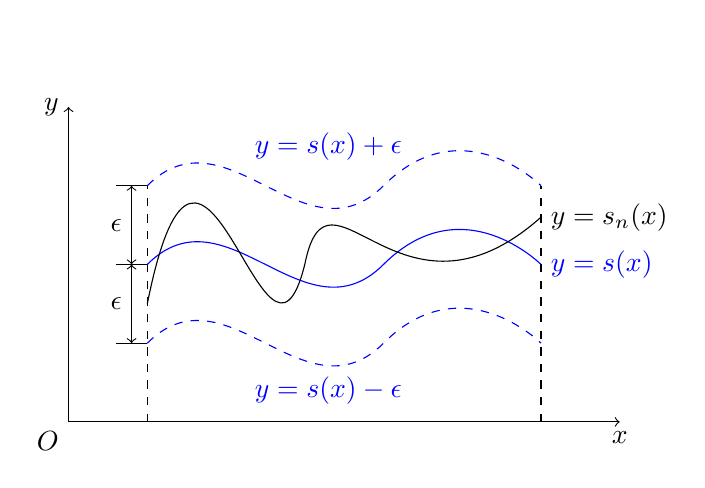
\begin{tikzpicture}
\draw[->](0,0)node[below left]{\(O\)} -- (7,0)node[below]{\(x\)};
\draw[->](0,0) -- (0,4)node[left]{\(y\)};
\draw[dashed](1,0) -- (1,3) (6,0) -- (6,3);
\draw(1,1)--+(-.4,0);
\draw(1,2)--+(-.4,0);
\draw(1,3)--+(-.4,0);
\begin{scope}[<->,xshift=-.2cm]
\draw(1,1) -- (1,2)node[midway,left]{\(\epsilon\)};
\draw(1,2) -- (1,3)node[midway,left]{\(\epsilon\)};
\end{scope}
\begin{scope}[blue]
\draw[dashed] (1,1) .. controls (2,2) and (3,0) .. (4,1) .. controls (5,2) and (6,1) .. (6,1);
\draw[yshift=1cm] (1,1) .. controls (2,2) and (3,0) .. (4,1) .. controls (5,2) and (6,1) .. (6,1)node[right]{\(y = s(x)\)};
\draw[yshift=2cm,dashed] (1,1) .. controls (2,2) and (3,0) .. (4,1) .. controls (5,2) and (6,1) .. (6,1);
\draw(3.3,3.5)node{\(y = s(x) + \epsilon\)};
\draw(3.3,0.4)node{\(y = s(x) - \epsilon\)};
\end{scope}
\draw(1,1.5) .. controls (1.7,5) and (2.5,0) .. (3,2) .. controls (3.3,3.5) and (4.2,1) .. (6,2.6)node[right]{\(y = s_n(x)\)};
\end{tikzpicture}
\caption{函数项级数一致收敛的几何解释}
\label{figure:无穷级数.函数项级数一致收敛的几何解释}
\end{figure}

\begin{example}
研究级数\[
\frac{1}{x+1} + \left(\frac{1}{x+2}-\frac{1}{x+1}\right)
+ \dotsb + \left(\frac{1}{x+n}-\frac{1}{x+n-1}\right) + \dotsb
\]在区间\([0,+\infty)\)上的一致收敛性.
\begin{solution}
级数的前n项和\(s_n(x) = \frac{1}{x+n}\),因此级数的和\[
s(x) = \lim\limits_{n\to\infty} s_n(x) = \lim\limits_{n\to\infty} \frac{1}{x+n} = 0
\quad(0 \leq x < +\infty).
\]于是,余项的绝对值\[
\abs{r_n(x)} = \abs{s(x) - s_n(x)}
= \frac{1}{x+n} \leq \frac{1}{n}
\quad(0 \leq x < +\infty).
\]\(\forall\epsilon>0\),取\(N \geq \frac{1}{\epsilon}\),则当\(n>N\)时,\(\forall x\in[0,+\infty)\),有\(\abs{r_n(x)} < \epsilon\).根据定义,所给级数在区间\([0,+\infty)\)上一致收敛于\(s(x)\equiv0\).
\end{solution}
\end{example}

\begin{example}
研究级数\[
x + (x^2-x) + \dotsb + (x^n-x^{n-1}) + \dotsb
\]在区间\((0,1)\)上的一致收敛性.
\begin{solution}
这级数在区间\((0,1)\)内处处收敛于和\(s(x)\equiv0\),但并不一致收敛.事实上,这个级数的部分和\(s_n(x) = x^n\).\(\forall n\in\mathbb{N}^+\),取\(x_n = \frac{1}{\sqrt[n]{2}}\),于是\[
s_n(x_n) = x_n^n = \frac{1}{2},
\]但\(s(x_n) = 0\),从而\[
\abs{r_n(x_n)} = \abs{s(x_n) - s_n(x_n)} = \frac{1}{2}.
\]所以,只要取\(\epsilon<\frac{1}{2}\),不论\(n\)多么大,在\((0,1)\)内总存在这样的点\(x_n\),使得\(\abs{r_n(x_n)}>\epsilon\),因此所给级数在\((0,1)\)内不一致收敛.

这表明虽然函数序列\(s_n(x) = x^n\)在\((0,1)\)内处处收敛于\(s(x)\equiv0\),但\(s_n(x)\)在\((0,1)\)内各点处收敛于零的“快慢”程度是不一致的.

可是\(\forall r\in(0,1)\),这级数在\([0,r]\)上一致收敛.这是因为当\(x=0\)时,显然\[
\abs{r_n(x)} = x^n = 0 < \epsilon;
\]当\(0 < x \leq r\)时,要使\(x^n < \epsilon\)(不妨设\(\epsilon < 1\)),只要\(n \ln x < \ln\epsilon\)或\(n > \frac{\ln\epsilon}{\ln x}\);而\(\frac{\ln\epsilon}{\ln x}\)在\((0,r]\)上的最大值为\(\frac{\ln\epsilon}{\ln r}\),故取正整数\(N \geq \frac{\ln\epsilon}{\ln r}\),则当\(n > N\)时,对\([0,r]\)上的一切\(x\)都有\(x^n < \epsilon\).
\end{solution}
\end{example}
上例说明了一致收敛性与所讨论的区间有关.

\subsection{魏尔斯特拉斯判别法}
以上两例都是直接根据定义来判定级数的一致收敛性的,现在介绍一个在实用上较方便的判别法.
\begin{theorem}[魏尔斯特拉斯判别法]\label{theorem:无穷级数.魏尔斯特拉斯判别法}
如果函数项级数\(\sum\limits_{n=1}^\infty u_n(x)\)在区间\(I\)上满足条件\begin{enumerate}
\item \(\abs{u_n(x)} \leq a_n \quad(n=1,2,\dotsc)\);
\item 正项级数\(\sum\limits_{n=1}^\infty a_n\)收敛,
\end{enumerate}
则函数项级数\(\sum\limits_{n=1}^\infty u_n(x)\)在区间\(I\)上一致收敛.
\begin{proof}
由条件2,根据\hyperref[theorem:无穷级数.级数的柯西审敛原理]{柯西审敛原理},
\(\forall\epsilon>0\),\(\exists N \in \mathbb{N}^+\),
使得当\(n > N\)时,\(\forall p \in \mathbb{N}^+\),都有\[
a_{n+1} + a_{n+2} + \dotsb + a_{n+p} < \frac{\epsilon}{2}.
\]由条件1,\(\forall x \in I\),都有\begin{align*}
&\hspace{-20pt}\abs{u_{n+1}(x) + u_{n+2}(x) + \dotsb + u_{n+p}(x)} \\
&\leq \abs{u_{n+1}(x)} + \abs{u_{n+2}(x)} + \dotsb + \abs{u_{n+p}(x)} \\
&\leq a_{n+1} + a_{n+2} + \dotsb + a_{n+p} < \frac{\epsilon}{2},
\end{align*}令\(p\to\infty\),则由上式得\[
\abs{r_n(x)} \leq \frac{\epsilon}{2} < \epsilon.
\]因此函数项级数\(\sum\limits_{n=1}^\infty u_n(x)\)在区间\(I\)上一致收敛.
\end{proof}
\end{theorem}

\begin{example}
证明级数\[
\frac{\sin x}{1^2}
+ \frac{\sin 2^2 x}{2^2}
+ \dotsb
+ \frac{\sin n^2 x}{n^2}
+ \dotsb
\]在区间\((-\infty,+\infty)\)内一致收敛.
\begin{proof}
因为在\((-\infty,+\infty)\)内\[
\abs{\frac{\sin n^2 x}{n^2}} \leq \frac{1}{n^2}
\quad(n=1,2,\dotsc),
\]而\(\sum\limits_{n=1}^\infty \frac{1}{n^2}\)收敛,
故由\hyperref[theorem:无穷级数.魏尔斯特拉斯判别法]{魏尔斯特拉斯判别法},
所给级数在\((-\infty,+\infty)\)内一致收敛.
\end{proof}
\end{example}

\subsection{阿贝尔判别法}
\begin{theorem}[阿贝尔判别法]\label{theorem:无穷级数.阿贝尔判别法}
如果有
\begin{enumerate}
\item 函数项级数\(\sum\limits_{n=1} a_n(x)\)在区间\(I\)上一致收敛;
\item 函数\(b_n(x)\ (n=1,2,\dotsc)\)都有界,且对任意\(x\)组成一个单调序列;
\end{enumerate}
那么函数项级数\[
	\sum\limits_{n=1} a_n(x) b_n(x)
\]
在区间\(I\)上一致收敛.
\end{theorem}

\subsection{狄利克雷判别法}
\begin{theorem}[狄利克雷判别法]\label{theorem:无穷级数.狄利克雷判别法}
如果有
\begin{enumerate}
\item 部分和\(\sum\limits_{i=1}^n a_i(x)\)总是有界的;
\item 序列\(\{b_n(x)\}\)对于任意\(x\)都是单调的,
且当\(n\to\infty\)时在区间\(I\)上一致地趋于零;
\end{enumerate}
那么函数项级数\[
	\sum\limits_{n=1} a_n(x) b_n(x)
\]
在区间\(I\)上一致收敛.
\end{theorem}

\subsection{一致收敛级数的基本性质}
一致收敛级数有如下基本性质.
\begin{property}\label{theorem:无穷级数.一致收敛级数的基本性质1}
\def\su{\sum\limits_{n=1}^\infty u_n(x)}
如果级数\(\su\)的各项\(u_n(x)\)在区间\([a,b]\)上都连续,且\(\su\)在区间\([a,b]\)上一致收敛于\(s(x)\),则\(s(x)\)在\([a,b]\)上也连续.
\begin{proof}
设\(x_0,x\)是\([a,b]\)上任意两点.由等式\[
s(x) = s_n(x) + r_n(x),
\qquad
s(x_0) = s_n(x_0) + r_n(x_0)
\]得\begin{align*}
\abs{s(x) - s_(x_0)}
&= \abs{s_n(x) - s_n(x_0) + r_n(x) - r_n(x_0)} \\
&\leq \abs{s_n(x) - s_n(x_0)} + \abs{r_n(x)} + \abs{r_n(x_0)}.
\tag1
\end{align*}
因为级数\(\su\)一致收敛于\(s(x)\),所以\(\forall\epsilon>0\),必有正整数\(N = N(\epsilon)\),使得当\(n>N\)时,\(\forall x \in [a,b]\),都有\[
\abs{r_n(x)} < \frac{\epsilon}{3}.
\eqno{(2)}
\]当然,也有\(\abs{r_n(x_0)} < \frac{\epsilon}{3}\).选定满足大于\(N\)的\(n\)之后,\(s_n(x)\)是有限项连续函数之和,故\(s_n(x)\)在点\(x_0\)连续,从而必有一个\(\delta > 0\)存在,当\(\abs{x - x_0} < \delta\)时,总有\[
\abs{s_n(x) - s_n(x_0)} < \frac{\epsilon}{3}.
\eqno{(3)}
\]由(1)、(2)、(3)式可见,对任给\(\epsilon>0\),必有\(\delta > 0\),当\(\abs{x - x_0} < \delta\)时,有\[
\abs{s(x) - s(x_0)} < \epsilon.
\]所以\(s(x)\)在点\(x_0\)处连续,而\(x_0\)在\([a,b]\)上是任意的,因此\(s(x)\)在\([a,b]\)上连续.
\end{proof}
\end{property}

\begin{property}\label{theorem:无穷级数.一致收敛级数的基本性质2}
若函数项级数\(\sum\limits_{n=1}^\infty u_n(x)\)在区间\(I\)上内闭一致收敛,且\[
\lim\limits_{x \to a} u_n(x) = A_n
\quad(n=1,2,\dotsc),
\]
则级数\(\sum\limits_{n=1}^\infty A_n\)收敛,且\[
\lim\limits_{x \to a} \left\{
	\sum\limits_{n=1}^\infty u_n(x)
\right\}
= \sum\limits_{n=1}^\infty \left\{
	\vphantom{\sum\limits_{n=1}^\infty }
	\lim\limits_{x \to a} u_n(x)
\right\}.
\]
\end{property}

\begin{property}\label{theorem:无穷级数.一致收敛级数的基本性质3}
如果级数\(\sum\limits_{n=1}^\infty u_n(x)\)的各项\(u_n(x)\)在区间\([a,b]\)上都连续,
且\(\sum\limits_{n=1}^\infty u_n(x)\)在区间\([a,b]\)上一致收敛于\(s(x)\),
则级数\(\sum\limits_{n=1}^\infty u_n(x)\)在\([a,b]\)上可以逐项积分,
即\[
	\int_{x_0}^x s(x) \dd{x}
	= \sum\limits_{n=1}^\infty \int_{x_0}^x u_n(x) \dd{x},
\]
其中\(a \leq x_0 < x \leq b\),并且上式右端的级数在\([a,b]\)上也一致收敛.
\begin{proof}
因为级数\(\sum\limits_{n=1}^\infty u_n(x)\)在\([a,b]\)上一致收敛,
由\cref{theorem:无穷级数.一致收敛级数的基本性质1},
\(s(x)\)和\(r_n(x)\)都在\([a,b]\)上连续,
所以积分\(\int_{x_0}^x s(x) \dd{x}\)和\(\int_{x_0}^x r_n(x) \dd{x}\)存在,
从而\[
	\abs{\int_{x_0}^x s(x) \dd{x} - \int_{x_0}^x s_n(x) \dd{x}}
	= \abs{\int_{x_0}^x r_n(x) \dd{x}}
	\leq \int_{x_0}^x \abs{r_n(x)} \dd{x}.
\]
又由级数的一致收敛性,
\(\forall\epsilon>0\),
\(\exists N = N(\epsilon) \in \mathbb{N}^+\),
使得当\(n > N\)时,
\(\forall x \in [a,b]\),
都有\[
	\abs{r_n(x)} < \frac{\epsilon}{b-a}.
\]
于是,当\(n > N\)时,有\[
	\abs{\int_{x_0}^x s(x) \dd{x} - \int_{x_0}^x s_n(x) \dd{x}}
	\leq \int_{x_0}^x \abs{r_n(x)} \dd{x}
	< \frac{\epsilon}{b-a} \cdot (x-x_0)
	\leq \epsilon.
\]
根据极限的定义,有\[
	\int_{x_0}^x s(x) \dd{x}
	= \lim\limits_{n\to\infty} \int_{x_0}^x s_n(x) \dd{x}
	= \lim\limits_{n\to\infty} \sum\limits_{i=1}^n \int_{x_0}^x u_i(x) \dd{x}
	= \sum\limits_{n=1}^\infty \int_{x_0}^x u_n(x) \dd{x}.
\]
由于\(N\)只依赖于\(\epsilon\)而与\(x_0,x\)无关,
所以级数\(\sum\limits_{n=1}^\infty \int_{x_0}^x u_n(x) \dd{x}\)在\([a,b]\)上一致收敛.
\end{proof}
\end{property}

\begin{property}\label{theorem:无穷级数.一致收敛级数的基本性质4}
如果级数\(\sum\limits_{n=1}^\infty u_n(x)\)的各项\(u_n(x)\)都具有连续导数\(u'_n(x)\),
且\(\sum\limits_{n=1}^\infty u_n(x)\)在区间\([a,b]\)上收敛于和\(s(x)\),
它并且级数\(\sum\limits_{n=1} u'_n(x)\)在\([a,b]\)上一致收敛,
则级数\(\sum\limits_{n=1}^\infty u_n(x)\)在区间\([a,b]\)上也一致收敛,且可逐项求导,
即\[
	s'(x) = \sum\limits_{n=1} u'_n(x).
\]
\begin{proof}
由于\(\sum\limits_{n=1} u'_n(x)\)在\([a,b]\)上一致收敛,设其和为\(v(x)\),即\[
	\sum\limits_{n=1} u'_n(x) = v(x).
\]
根据\cref{theorem:无穷级数.一致收敛级数的基本性质1} 知,
\(v(x)\)在\([a,b]\)上连续.
再根据\cref{theorem:无穷级数.一致收敛级数的基本性质3},
级数\(\sum\limits_{n=1} u'_n(x)\)可逐项积分,故\[
	\int_{x_0}^x v(x) \dd{x}
	= \sum\limits_{n=1} \int_{x_0}^x u'_n(x) \dd{x}
	= \sum\limits_{n=1} [u_n(x) - u_n(x_0)],
\]
而\(\sum\limits_{n=1}^\infty u_n(x) = s(x)\),
\(\sum\limits_{n=1}^\infty u_n(x_0) = s(x_0)\),
故\[
	\sum\limits_{n=1} [u_n(x) - u_n(x_0)]
	= s(x) - s(x_0),
\]
从而有\[
	\int_{x_0}^x v(x) \dd{x} = s(x) - s(x_0),
\]
其中\(a \leq x_0 < x \leq b\).
上式两端求导,即得关系式\[
	v(x) = s'(x).
\]

根据\cref{theorem:无穷级数.一致收敛级数的基本性质3},
级数\(\sum\limits_{n=1} \int_{x_0}^x u'_n(x) \dd{x}\)在\([a,b]\)上一致收敛,而\[
	\sum\limits_{n=1} \int_{x_0}^x u'_n(x) \dd{x}
	= \sum\limits_{n=1}^\infty u_n(x)
		- \sum\limits_{n=1}^\infty u_n(x_0),
\]所以\[
	\sum\limits_{n=1}^\infty u_n(x)
	= \sum\limits_{n=1} \int_{x_0}^x u'_n(x) \dd{x}
	+ \sum\limits_{n=1}^\infty u_n(x_0).
\]也就是说,级数\(\sum\limits_{n=1}^\infty u_n(x)\)在\([a,b]\)上一致收敛.
\end{proof}
\end{property}

\section{幂级数}
\subsection{幂级数的概念}
\begin{definition}\label{definition:无穷级数.幂级数}
各项均是幂函数的函数项级数,
称为\DefineConcept{幂级数}(power series).

称级数\[
\sum\limits_{i=0}^\infty a_i (x-x_0)^i
= a_0 + a_1 (x-x_0) + a_2 (x-x_0)^2 + \dotsb + a_n (x-x_0)^n + \dotsb,
\]为“幂级数的\DefineConcept{一般形式}”.
称级数\[
\sum\limits_{n=0}^\infty a_n x^n
= a_0 + a_1 x + a_2 x^2 + \dotsb + a_n x^n + \dotsb,
\]为“幂级数的\DefineConcept{标准形式}”.
这里常数\(a_0,\AutoTuple{a}{n},\dotsc\)称为幂级数的\DefineConcept{系数}.
\end{definition}

由于幂级数的一般形式只要作变量代换\(t = x - x_0\)就可化为它的标准形式,
因此,即便我们取标准形式来讨论,也并不影响一般性.

\subsection{幂级数的收敛性}
现在我们来讨论:
对于一个给定的幂级数,
它的收敛域与发散域是怎样的?
即\(x\)取数轴上哪些点时幂级数收敛,
取哪些点时幂级数发散?
这就是幂级数的收敛性问题.

先看一个例子.
\begin{example}
考察幂级数\[
1+x^2+x^3+\dotsb+x^n+\dotsb
\]的收敛性.
我们已经知道,当\(\abs{x}<1\)时,该级数收敛于\(\frac{1}{1-x}\);
当\(\abs{x}\geq1\)时,该级数发散.
因为,这个幂级数的收敛域是开区间\((-1,1)\),发散域是\((-\infty,-1]\cup[1,+\infty)\),并有\[
\frac{1}{1-x} = 1+x+x^2+\dotsb+x^n+\dotsb
\quad(-1<x<1).
\]
\end{example}

在这个例子中我们看到,这个幂级数的收敛域是一个区间.
事实上,这个结论对于一般的幂级数也是成立的.
我们有如下的定理.

\begin{theorem}[阿贝尔定理]\label{theorem:无穷级数.阿贝尔定理}
如果级数\(\sum\limits_{n=0}^\infty a_n x^n\)当\(x=x_0\neq0\)时收敛,
则满足\(\abs{x}<\abs{x_0}\)的一切\(x\)可使该幂级数绝对收敛.
反之,如果级数\(\sum\limits_{n=0}^\infty a_n x^n\)当\(x=x_0\)时发散,
则满足\(\abs{x}>\abs{x_0}\)的一切\(x\)均使该幂级数发散.
\begin{proof}
先设\(x_0\neq0\)是幂级数\(\sum\limits_{n=1}^\infty a_n x^n\)的收敛点,
即常数项级数\[
a_0 + a_1 x_0 + a_2 x_0^2 + \dotsb + a_n x_0^n + \dotsb
\]收敛.
根据级数收敛的必要条件,这时有\[
\lim\limits_{n\to\infty} a_n x_0^n = 0;
\]
于是\(\exists M > 0\),使得\[
	\abs{a_n x_0^n} \leq M
	\quad(n=0,1,2,\dotsc).
\]
这样幂级数\(\sum\limits_{n=1}^\infty a_n x^n\)的一般项的绝对值\[
	\abs{a_n x^n} = \abs{a_n x_0^n \cdot \frac{x^n}{x_0^n}}
	= \abs{a_n x_0^n} \cdot \abs{\frac{x}{x_0}}^n
	\leq M \abs{\frac{x}{x_0}}^n.
\]
因为当\(\abs{x}<\abs{x_0}\)时,
等比级数\(\sum\limits_{n=0}^\infty M \abs{\frac{x}{x_0}}^n\)收敛,
所以级数\(\sum\limits_{n=1} \abs{a_n x^n}\)收敛,
也就是级数\(\sum\limits_{n=1}^\infty a_n x^n\)绝对收敛.

定理的第二部分可用反证法证明.
假设幂级数当\(x=x_0\)时发散而有一点\(x_1\)适合\(\abs{x_1}>\abs{x_0}\)使级数收敛,
则根据本定理的第一部分,当\(x=x_0\)时级数应收敛,这与假设矛盾.
\end{proof}
\end{theorem}

\cref{theorem:无穷级数.阿贝尔定理} 表明,
如果幂级数在\(x=x_0\)处收敛,
则对\(\forall x\in(-\abs{x_0},\abs{x_0})\),幂级数都收敛;
如果幂级数在\(x=x_0\)处发散,
则对\(\forall x\in\mathbb{R}-[-\abs{x_0},\abs{x_0}]\),幂级数都发散.

设已给幂级数在数轴上既有收敛点(不仅是原点)也有发散点.
现在从原点出发沿数轴正方向走,最初只遇到收敛点,然后就只遇到发散点.
这两部分的界点可能是收敛点,也可能是发散点.
从原点出发沿数轴负方向走,情形相同.
利用\cref{theorem:无穷级数.阿贝尔定理} 可以证明:原点两侧的两个界点到原点的距离是相等的.
像这样,我们就得到以下重要推论.
\begin{corollary}\label{theorem:无穷级数.阿贝尔定理推论}
如果幂级数\(\sum\limits_{n=0}^\infty a_n x^n\)不是仅在\(x=0\)一点收敛,也不是在整个数轴上都收敛,则必定存在正数\(R\),使得:\begin{enumerate}
\item 当\(\abs{x}<R\)时,幂级数绝对收敛;
\item 当\(\abs{x}>R\)时,幂级数发散;
\item 当\(\abs{x}=R\)时,幂级数可能收敛也可能发散.
\end{enumerate}
\end{corollary}

我们称\cref{theorem:无穷级数.阿贝尔定理推论} 中提到的正数\(R\)为“幂级数的\DefineConcept{收敛半径}”.
称开区间\((-R,R)\)为“幂级数的\DefineConcept{收敛区间}”.

在已知幂级数的收敛半径或收敛区间的情况下,
我们可以根据幂级数在点\(x = \pm R\)处的收敛性,
就可以决定其收敛域是\((-R,R)\)、\([-R,R)\)、\((-R,R]\)或\([-R,R]\)四个区间之一.

如果幂级数只在\(x=0\)处收敛,这时收敛域为\(\{0\}\),规定收敛半径\(R=0\).
如果幂级数对任意实数都收敛,则规定收敛半径\(R=+\infty\),收敛域为\((-\infty,+\infty)\).

关于幂级数的收敛半径的求法,有下面的定理.
\begin{theorem}\label{theorem:无穷级数.幂级数的收敛半径的求法}
如果\[
\lim\limits_{n\to\infty} \abs{\frac{a_{n+1}}{a_n}} = \rho,
\]其中\(a_n\)、\(a_{n+1}\)是幂级数\(\sum\limits_{i=0}^\infty {a_i x^i}\)的相邻两项的系数,
则这幂级数的收敛半径为\[
\def\arraystretch{1.5}
R = \left\{ \begin{array}{ll}
\frac{1}{\rho}, & \rho \in (0,+\infty), \\
+\infty, & \rho = 0, \\
0, & \rho = +\infty \\
\end{array} \right.
\]或\[
R = \lim\limits_{n\to\infty} {\abs{\frac{a_n}{a_{n+1}}}}.
\]
\begin{proof}
\def\s{\sum\limits_{n=0}^\infty }%
考察幂级数\(\sum\limits_{n=1} a_n x^n\)的各项取绝对值所成的级数\[
	\sum\limits_{n=1} \abs{a_n x^n}
	= \abs{a_0} + \abs{a_1 x} + \abs{a_2 x^2} + \dotsb + \abs{a_n x^n} + \dotsb.
\]
这级数相邻两项之比为\[
	\frac{\abs{a_{n+1} x^{n+1}}}{\abs{a_n x^n}}
	= \abs{\frac{a_{n+1}}{a_n}} \abs{x}.
\]

\begin{enumerate}
	\item 如果极限\(\lim\limits_{n\to\infty} \abs{\frac{a_{n+1}}{a_n}} = \rho\neq0\)存在,
	根据\hyperref[theorem:无穷级数.正项级数的比值审敛法]{比值审敛法},
	则当\(\rho \abs{x} < 1\)即\(\abs{x} < \frac{1}{\rho}\)时,
	级数\(\sum\limits_{n=1} \abs{a_n x^n}\)收敛,
	从而级数\(\sum\limits_{n=1} a_n x^n\)绝对收敛;
	再根据\cref{theorem:无穷级数.绝对发散的特殊情况},
	当\(\rho \abs{x} > 1\)即\(\abs{x} > \frac{1}{\rho}\)时,
	级数\(\sum\limits_{n=1} \abs{a_n x^n}\)发散,
	并且\[
		(\exists N\in\mathbb{N})
		(\forall n\in\mathbb{N})
		[
			n > N
			\implies
			\abs{a_{n+1} x^{n+1}} > \abs{a_n x^n}
		].
	\]

	\item 如果\(\rho=0\),
	则对\(\forall x\neq0\),
	有\(\lim\limits_{n\to\infty} \abs{\frac{a_{n+1} x^{n+1}}{a_n x^n}} = 0\),
	所以级数\(\sum\limits_{n=1} \abs{a_n x^n}\)收敛,
	从而级数\(\sum\limits_{n=1} a_n x^n\)绝对收敛.
	于是\(R=+\infty\).
		\item 如果\(\rho=+\infty\),
	则对\(\forall x\neq0\),
	级数\(\sum\limits_{n=1} a_n x^n\)必发散,
	否则由\cref{theorem:无穷级数.阿贝尔定理} 知道,
	\(\exists x\neq0\)使得\(\sum\limits_{n=1} \abs{a_n x^n}\)收敛.
	于是\(R=0\).
	\qedhere
\end{enumerate}
\end{proof}
\end{theorem}

\begin{example}
求幂级数\[
x-\frac{x^2}{2}+\frac{x^3}{3}-\dotsb+(-1)^{n-1}\frac{x^n}{n}+\dotsb
\]的收敛半径与收敛域.
\begin{solution}
因为\[
\rho = \lim\limits_{n\to\infty} \abs{\frac{a_{n+1}}{a_n}}
= \lim\limits_{n\to\infty} \frac{n}{n+1} = 1,
\]所以收敛半径\[
R = \frac{1}{\rho} = 1.
\]

对于端点\(x=1\),级数成为交错级数\[
1-\frac{1}{2}+\frac{1}{3}-\dotsb+(-1)^{n-1}\frac{1}{n}+\dotsb,
\]由\cref{example:无穷级数.交错级数1} 可知,此级数收敛;
对于端点\(x=-1\),级数成为\[
-1-\frac{1}{2}-\frac{1}{3}-\dotsb-\frac{1}{n}-\dotsb,
\]此级数发散.
综上所述,收敛域是\((-1,1]\).
\end{solution}
\end{example}
利用上例的结果可以计算出交错级数\[
1-\frac{1}{2}+\frac{1}{3}-\dotsb+(-1)^{n-1}\frac{1}{n}+\dotsb.
\]显然有
\begin{align*}
\sum\limits_{n=1}^\infty (-1)^{n-1} \frac{1}{n}
&= \eval{\sum\limits_{n=1}^\infty (-1)^{n-1} \frac{x^n}{n}}_{x=1} \\
&= \eval{\sum\limits_{n=1}^\infty (-1)^{n-1} \int_0^x \left(\frac{x^n}{n}\right)' \dd{x}}_{x=1} \\
&= \eval{\sum\limits_{n=1}^\infty (-1)^{n-1} \int_0^x x^{n-1} \dd{x}}_{x=1} \\
&= \eval{\int_0^x \sum\limits_{n=1}^\infty (-1)^{n-1} x^{n-1} \dd{x}}_{x=1} \\
&= \eval{\int_0^x \frac{1}{1+x} \dd{x}}_{x=1} \\
&= \eval{\ln(1+x)}_{x=1} = \ln2.
\end{align*}

\begin{example}
求幂级数\[
1+x+\frac{1}{2!}x^2+\dotsb+\frac{1}{n!}x^n+\dotsb
\]的收敛域.
\begin{solution}
因为\[
\rho = \lim\limits_{n\to\infty} \abs{\frac{a_{n+1}}{a_n}}
= \lim\limits_{n\to\infty} \frac{n!}{(n+1)!}
= \lim\limits_{n\to\infty} \frac{1}{n+1}
= 0,
\]所以收敛半径\(R = +\infty\),从而收敛域是\((-\infty,+\infty)\).
\end{solution}
\end{example}

\begin{example}
求幂级数\(\sum\limits_{n=0}^\infty n! x^n\)的收敛半径.
\begin{solution}
因为\[
\rho = \lim\limits_{n\to\infty} \abs{\frac{a_{n+1}}{a_n}}
= \lim\limits_{n\to\infty} \frac{(n+1)!}{n!} = +\infty,
\]所以收敛半径\(R = 0\),即级数仅在点\(x = 0\)处收敛.
\end{solution}
\end{example}

\begin{example}
求幂级数\(\sum\limits_{n=0}^\infty \frac{(2n)!}{(n!)^2} x^{2n}\)的收敛半径.
\begin{solution}
级数缺少奇次幂的项,\cref{theorem:无穷级数.幂级数的收敛半径的求法} 不能直接应用,
我们根据\cref{theorem:无穷级数.正项级数的比值审敛法的上下极限形式} 来求收敛半径:
\[
\lim\limits_{n\to\infty} \abs{{\frac{[2(n+1)]!}{[(n+1)!]^2} x^{2(n+1)}}\Bigg/{\frac{(2n)!}{(n!)^2} x^{2n}}}
= \lim\limits_{n\to\infty} \abs{\frac{(2n+2)(2n+1)}{(n+1)^2} x^2}
= 4 x^2.
\]

当\(4 x^2 < 1\)即\(\abs{x} < 1/2\)时级数收敛;
当\(4 x^2 > 1\)即\(\abs{x} > 1/2\)时级数发散.
所以收敛半径\(R = 1/2\).
\end{solution}
\end{example}

\begin{example}
求幂级数\(\sum\limits_{n=1}^\infty \frac{(x-1)^n}{2^n \cdot n}\)的收敛域.
\begin{solution}
令\(t = x-1\),上述级数变为\[
\sum\limits_{n=1}^\infty \frac{t^n}{2^n \cdot n}.
\]因为\[
\rho = \lim\limits_{n\to\infty} \abs{\frac{a_{n+1}}{a_n}} = \lim\limits_{n\to\infty} \frac{2^n \cdot n}{2^{n+1} \cdot (n+1)} = \frac{1}{2},
\]所以收敛半径\(R_t = 2\),而原级数的收敛区间为\(-1<x<3\).

当\(x=3\)时,级数成为\(\sum\limits_{n=1}^\infty \frac{1}{n}\),这级数发散;
当\(x=-1\)时,级数成为\(\sum\limits_{n=1}^\infty \frac{(-1)^n}{n}\),这级数收敛.
因此原级数的收敛域为\([-1,3)\).
\end{solution}
\end{example}

注意:当级数缺项时,不能直接运用以上定理求解幂级数的收敛半径,
而应该使用合适的审敛法(如比值审敛法、根值审敛法),或者对幂级数使用换元法.

\subsection{幂级数的运算}
设幂级数\[
\sum\limits_{n=0}^\infty a_n x^n
= a_0 + a_1 x + a_2 x^2 + \dotsb + a_n x^n + \dotsb
\]和\[
\sum\limits_{i=0}^\infty b_i x^i
= b_0 + b_1 x + b_2 x^2 + \dotsb + b_n x^n + \dotsb
\]分别在区间\((-R,R)\)和\((-R',R')\)内收敛.
对于这两个幂级数,可以进行下列四则运算:

\begin{definition}[幂级数的加法]
\(\left(\sum\limits_{n=0}^\infty a_n x^n\right)
+ \left(\sum\limits_{i=0}^\infty b_i x^i\right)
= \sum\limits_{i=0}^\infty (a_i+b_i) x^i\).
\end{definition}

\begin{definition}[幂级数的减法]
\(\left(\sum\limits_{n=0}^\infty a_n x^n\right)
- \left(\sum\limits_{i=0}^\infty b_i x^i\right)
= \sum\limits_{i=0}^\infty (a_i-b_i) x^i\).
\end{definition}

\begin{definition}[幂级数的乘法]
\(\left(\sum\limits_{n=0}^\infty a_n x^n\right)
\cdot \left(\sum\limits_{i=0}^\infty b_i x^i\right)
= \sum\limits_{i=0}^\infty \left(
	\sum\limits_{j=0}^{i} a_j b_{i-j}
\right) x^i\).
\end{definition}

\begin{definition}[幂级数的除法]
记\[
\frac{
	\sum\limits_{n=0}^\infty a_n x^n
}{
	\sum\limits_{i=0}^\infty b_i x^i
}
= \sum\limits_{i=0}^\infty c_i x^i,
\]假设\(b_0 \neq 0\).
为了决定系数\(c_0,c_1,\dotsc,c_n,\dotsc\),可以将级数\(\sum\limits_{i=0}^\infty b_i x^i\)与\(\sum\limits_{i=0}^\infty c_i x^i\)相乘,并令乘积中各项的系数分别等于级数\(\sum\limits_{n=0}^\infty a_n x^n\)中同次幂的系数,即得\[
\begin{array}{l}
a_0 = b_0 c_0, \\
a_1 = b_1 c_0 + b_0 c_1, \\
a_2 = b_2 c_0 + b_1 c_1 + b_0 c_2, \\
\hdotsfor{1} \\
\end{array}
\]由这些方程就可以顺序地求出\(c_0,c_1,\dotsc,c_n,\dotsc\).

相除后所得的幂级数\(\sum\limits_{i=0}^\infty c_i x^i\)的收敛区间可能比原来的两级数的收敛区间小得多.
\end{definition}

\subsection{幂级数的和函数的性质}
\begin{property}\label{theorem:无穷级数.一致收敛的幂级数的性质}
\def\s{\sum\limits_{n=0}^\infty }
如果幂级数\(\sum\limits_{n=1} a_n x^n\)的收敛半径为\(R>0\),则此级数在\((-R,R)\)内闭一致收敛.
\end{property}
进一步还可证明,如果幂级数\(\sum\limits_{n=0}^\infty a_n x^n\)在收敛区间的端点收敛,则一致收敛的区间可扩大到包含端点.

\begin{property}\label{theorem:无穷级数.幂级数的和函数的性质1}
幂级数\(\sum\limits_{n=0}^\infty a_n x^n\)的和函数\(s(x)\)在其收敛域\(I\)上连续.
\end{property}

关于和函数的连续性及逐项可积的结论,
由\cref{theorem:无穷级数.一致收敛级数的基本性质1,%
theorem:无穷级数.一致收敛级数的基本性质3,%
theorem:无穷级数.一致收敛的幂级数的性质}
立即可得.

\begin{property}\label{theorem:无穷级数.幂级数的和函数的性质2}
幂级数\(\sum\limits_{n=0}^\infty a_n x^n\)的和函数\(s(x)\)在其收敛域\(I\)上可积,并有逐项积分公式\[
\int_0^x s(x) \dd{x}
=\int_0^x \left[\sum\limits_{n=0}^\infty a_n x^n\right] \dd{x}
=\sum\limits_{i=0}^\infty \int_0^x a_i x^i \dd{x}
=\sum\limits_{i=0}^\infty \frac{a_i}{i+1} x^{i+1}.
\]

逐项积分后所得到的幂级数和原级数有相同的收敛半径、收敛域.
\end{property}

\begin{property}\label{theorem:无穷级数.幂级数的和函数的性质3}
\def\s{\sum\limits_{n=0}^\infty }
如果幂级数\(\sum\limits_{n=1} a_n x^n\)的收敛半径为\(R>0\),则其和函数\(s(x)\)在\((-R,R)\)内可导,且有逐项求导公式\[
s'(x)
= \left( \s a_n x^n \right)'
= \sum\limits_{n=0}^\infty (a_n x^n)'
= \sum\limits_{n=1}^\infty n a_n x^{n-1}.
\]逐项求导后所得到的幂级数与原级数具有相同的收敛半径.
\end{property}
逐项求导后所得到的幂级数虽然和原级数有相同的收敛半径,但可能有不同的收敛域,这是因为逐项求导后所得到的幂级数在边界点处的收敛性可能发生改变.

反复利用上述结论可得:幂级数\(\sum\limits_{n=0}^\infty a_n x^n\)的和函数\(s(x)\)在其收敛区间\((-R,R)\)内具有任意阶导数.


\begin{example}
求幂级数\(\sum\limits_{n=1} \frac{x^n}{n+1}\)的和函数.
\begin{solution}
先求收敛域.
由\[
	\lim\limits_{n\to\infty} \abs{\frac{a_{n+1}}{a_n}}
	= \lim\limits_{n\to\infty} \frac{n+1}{n+2}
	= 1,
\]得收敛半径\(R=1\).

在端点\(x = -1\)处,
幂级数成为\(\sum\limits_{n=1} \frac{(-1)^n}{n+1}\),
是收敛的交错级数;
在端点\(x = 1\)处,
幂级数成为\(\sum\limits_{n=1} \frac{1}{n+1}\),
是发散的.
因此收敛域是\(I = [-1,1)\).

设和函数为\(s(x)\),即\[
	s(x) = \sum\limits_{n=1} \frac{x^n}{n+1},
	\quad x\in[-1,1).
\]
于是\[
	x s(x) = \sum\limits_{n=1} \frac{x^{n+1}}{n+1}.
\]

利用\cref{theorem:无穷级数.幂级数的和函数的性质3},逐项求导,并由\[
	\frac{1}{1-x} = 1+x+x^2+\dotsb+x^n+\dotsb
	\quad(-1<x<1),
\]
得\[
	[x s(x)]'
	= \sum\limits_{n=1} \left( \frac{x^{n+1}}{n+1} \right)'
	= \sum\limits_{n=1} x^n
	= \frac{1}{1-x}
	\quad(\abs{x}<1).
\]
对上式积分,
得\[
	x s(x) = \int_0^x \frac{1}{1-x} \dd{x} = -\ln(1-x)
	\quad(-1 \leq x < 1).
\]
于是,当\(x\neq0\)时,有\(s(x) = -\frac{1}{x} \ln(1-x)\).

而\(s(0)\)可由\(s(0) = a_0 = 1\)得出,
或者由和函数的连续性得到,即\[
	s(0)
	= \lim\limits_{x\to0} s(x)
	= \lim\limits_{x\to0} \left[ -\frac{1}{x} \ln(1-x) \right]
	= 1.
\]
故\[
	s(x) = \left\{ \begin{array}{cl}
		-\frac{1}{x} \ln(1-x), & x\in[-1,0)\cup(0,1), \\
		1, & x=0.
	\end{array} \right.
\]
\end{solution}
\end{example}

\section{函数展开成幂级数}
前面讨论了幂级数的收敛域及其和函数的性质.
但在许多应用中,我们遇到的却是相反的问题:
给定函数\(f(x)\),
要考虑它是否能在某个区间内“展开成幂级数”,
就是说,是否能找到这样一个幂级数,它在某区间内收敛,且其和恰好就是给定的函数\(f(x)\).
如果能找到这样的幂级数,我们就说“函数\(f(x)\)在该区间内能展开成幂级数”,
也说“这个幂级数在该区间内表达了函数\(f(x)\)”.

\subsection{泰勒展式}
\begin{definition}
设函数\(f(x)\)的定义域为\(D\).
如果在区间\(I \subseteq D\)内,
存在收敛的幂级数\(\sum\limits_{i=0}^\infty {a_i x^i}\)使得\[
f(x) = \sum\limits_{i=0}^\infty {a_i x^i}
\quad(x \in I)
\]成立,则称“函数\(f(x)\)在区间\(I\)内能展开成幂级数”.
\end{definition}

\begin{definition}
级数\[
\sum\limits_{n=0}^\infty \frac{1}{n!} f^{(n)}(x_0) (x-x_0)^n
\]
为“函数\(f(x)\)在点\(x_0\)处的\DefineConcept{泰勒级数}(Taylor series)”.

等式\[
f(x) = \sum\limits_{n=0}^\infty {\frac{1}{n!} f^{(n)}(x_0) (x-x_0)^n},
\quad x \in U(x_0).
\]称为函数\(f(x)\)在点\(x_0\)处的\DefineConcept{泰勒展开式}.
\end{definition}

可以看出,函数\(f(x)\)在\(U(x_0)\)内能展开成幂级数的充要条件为:
泰勒级数\[
\sum\limits_{n=0}^\infty {\frac{1}{n!} f^{(n)}(x_0) (x-x_0)^n}
\]在\(U(x_0)\)内收敛,且收敛到\(f(x)\).
但是“泰勒级数收敛到函数\(f(x)\)”这一叙述非常模糊,所以我们有以下定理:
\begin{theorem}
设函数\(f(x)\)在点\(x_0\)的某一邻域\(U(x_0)\)内具有各阶导数,
则\(f(x)\)在该邻域内能展开成泰勒级数的充要条件是:
在该邻域内\(f(x)\)的泰勒公式中的余项\(R_n(x)\)满足\[
\lim\limits_{n\to\infty} R_n(x) = 0,
\quad x \in U(x_0).
\]
\end{theorem}

\begin{definition}
级数\[
\sum\limits_{n=0}^\infty \frac{1}{n!} f^{(n)}(0) x^n
\]称为函数\(f(x)\)的\DefineConcept{麦克劳林级数}.

等式\[
f(x) = \sum\limits_{n=0}^\infty {\frac{1}{n!} f^{(n)}(0) x^n}
\quad(\abs{x} < r)
\]称为函数\(f(x)\)的\DefineConcept{麦克劳林展开式}.
\end{definition}

\begin{theorem}
若函数\(f(x)\)在区间\(I\)内能展开成幂级数,
则它的幂级数展开式是唯一的.
\end{theorem}

{\color{red}
要把函数\(f(x)\)展开成麦克劳林级数,可以按照下列步骤进行:
\begin{enumerate}
\item 求出函数\(f(x)\)的各阶导数\[
f'(x),f''(x),\dotsc,f^{(n)}(x),\dotsc.
\]如果在\(x=0\)处某阶导数不存在,就停止展开,因为这就说明函数\(f(x)\)不能展开为麦克劳林级数.
\item 求出函数及其各阶导数在\(x=0\)处的值:\[
f(0),f'(0),f''(0),\dotsc,f^{(n)}(0),\dotsc.
\]
\item 写出幂级数\[
f(0) + f'(0) x + \frac{f''(0)}{2!} x^2 + \dotsb + \frac{f^{(n)}(0)}{n!} x^n + \dotsb,
\]并求出收敛半径\(R\).
\item 利用余项\(R_n(x)\)的表达式\[
R_n(x) = \frac{1}{(n+1)!} f^{(n+1)}(\theta x) x^{n+1}
\quad(0 < \theta < 1),
\]考察当\(x\)在区间\((-R,R)\)内时余项的极限\(\lim\limits_{n\to\infty} R_n(x)\)是否为零.

如果\(\lim\limits_{n\to\infty} R_n(x) = 0\),则函数\(f(x)\)在区间\((-R,R)\)内的麦克劳林展开式为\[
f(x) = \sum\limits_{n=0}^\infty \frac{1}{n!} f^{(n)}(0) x^n
\quad(-R < x < R).
\]

如果\(\lim\limits_{n\to\infty} R_n(x) \neq 0\),则函数\(f(x)\)不能展开为麦克劳林级数.
\end{enumerate}
}

需要注意的是,不要错误地认为“如果一个函数的泰勒级数在点\(x_0\)处收敛,那么该级数就一定收敛到这个函数”.
\begin{example}\label{example:无穷级数.函数的泰勒级数不一定收敛到函数}
最常见的例子是:\[
f(x) = \left\{ \begin{array}{ll}
e^{-1/x^2}, & x\neq0, \\
0, & x=0.
\end{array} \right.
\]
根据导数的定义,以及\(\forall k\in\mathbb{R}: x^k e^{-1/x^2} \to 0\ (x\to0)\),
可知\(f^{(n)}(0) = 0\ (n=0,1,2,\dotsc)\).
于是,函数\(f\)在点\(x=0\)处的泰勒级数的每一项都是零,其和恒等于零;
只不过,当\(x\neq0\)时,\(f(x)\neq0\).
\end{example}

\begin{example}
将函数\(f(x) = e^x\)展开成\(x\)的幂级数.
\begin{solution}
所给函数的各阶导数为\[
f^{(n)}(x) = e^x
\quad(n=1,2,\dotsc),
\]因此\[
f^{(n)}(x) = 1
\quad(n=0,1,2,\dotsc).
\]于是得级数\[
1+x+\frac{x^2}{2!}+\dotsb+\frac{x^n}{n!}+\dotsb,
\]它的收敛半径\(R = +\infty\).

对于任何有限的数\(x\)和\(\xi\)(\(\xi\)在\(0\)与\(x\)之间),余项的绝对值为\[
\abs{R_n(x)} = \abs{\frac{e^{\xi}}{(n+1)!} x^{n+1}}
< e^{\abs{x}} \cdot \frac{\abs{x}^{n+1}}{(n+1)!}.
\]因为\(e^{\abs{x}}\)有限,而\(\frac{\abs{x}^{n+1}}{(n+1)!}\)是收敛级数\(\sum\limits_{n=0}^\infty \frac{\abs{x}^{n+1}}{(n+1)!}\)的一般项,所以当\(n\to\infty\)时,\(e^{\abs{x}} \cdot \frac{\abs{x}^{n+1}}{(n+1)!}\to0\),即\[
\lim\limits_{n\to\infty} \abs{R_n(x)} = 0.
\]于是得展开式\[
e^x = 1+x+\frac{x^2}{2!}+\dotsb+\frac{x^n}{n!}+\dotsb
\quad(-\infty<x<+\infty).
\]
\end{solution}
\end{example}

\begin{example}
将函数\(f(x) = \sin x\)展开成\(x\)的幂级数.
\begin{solution}
所给函数的各阶导数为\[
f^{(n)}(x) = \sin\left(x + n\cdot\frac{\pi}{2}\right)
\quad(n=1,2,\dotsc),
\]易见\(f^{(n)}(0)\)依顺序循环地取\(0,1,0,-1,\dotsc\),于是得级数\[
x-\frac{x^3}{3!}+\frac{x^5}{5!}-\dotsb+(-1)^k \frac{x^{2k+1}}{(2k+1)!}+\dotsb,
\]它的收敛半径\(R=+\infty\).

对于任何有限的数\(x\)和\(\xi\)(\(\xi\)在\(0\)与\(x\)之间),余项的绝对值为\[
\abs{R_n(x)}
= \abs{ \frac{x^{n+1}}{(n+1)!} \sin\left[\xi+\frac{n+1}{2}\pi\right] }
\leq \frac{\abs{x}^{n+1}}{(n+1)!}.
\]而\[
\lim\limits_{n\to\infty} \frac{\abs{x}^{n+1}}{(n+1)!} = 0.
\]因而得展开式\[
\sin x = x-\frac{x^3}{3!}+\frac{x^5}{5!}-\dotsb+(-1)^k \frac{x^{2k+1}}{(2k+1)!}+\dotsb
\quad(-\infty<x<+\infty).
\]
\end{solution}
\end{example}

以上将函数展开成幂级数的例子,是直接按公式\[
a_n = \frac{1}{n!} f^{(n)}(0)
\]计算幂级数的系数,最后考察余项\(R_n(x)\)是否趋于零.
这种直接展开的方法计算量较大,而且研究余项即使在初等函数中也不是一件容易的事.
下面介绍间接展开的方法,这就是利用一些已知的函数展开式,通过幂级数的运算(如四则运算、逐项求导、逐项积分)以及变量代换等,将所给函数展开成幂级数.
这样做不但计算简单,而且可以避免研究余项.

前面我们已经求得的幂级数展开式有\begin{gather}
e^x = \sum\limits_{n=0}^\infty \frac{1}{n!} x^n
	\quad(-\infty<x<+\infty), \label{equation:无穷级数.幂级数展开式1} \\
\sin x = \sum\limits_{k=0}^\infty \frac{(-1)^k}{(2k+1)!} x^{2k+1}
	\quad(-\infty<x<+\infty), \label{equation:无穷级数.幂级数展开式2} \\
\frac{1}{1+x} = \sum\limits_{n=0}^\infty (-1)^n x^n
	\quad(-1<x<1). \label{equation:无穷级数.幂级数展开式3}
\end{gather}
利用这三个展开式,可以求得许多函数的幂级数展开式.
例如对\cref{equation:无穷级数.幂级数展开式3} 两边从\(0\)到\(x\)积分,可得
\begin{equation}\label{equation:无穷级数.幂级数展开式4}
\ln(1+x) = \sum\limits_{n=0}^\infty \frac{(-1)^n}{n+1} x^{n+1}
= \sum\limits_{n=1}^\infty \frac{(-1)^{n-1}}{n} x^n
\quad(-1<x\leq1);
\end{equation}

对\cref{equation:无穷级数.幂级数展开式2} 两边求导,即得
\begin{equation}\label{equation:无穷级数.幂级数展开式5}
\cos x = \sum\limits_{k=0}^\infty \frac{(-1)^k}{(2k)!} x^{2k}
\quad(-\infty<x<+\infty);
\end{equation}

把\cref{equation:无穷级数.幂级数展开式1} 中的\(x\)换成\(x \ln a\),可得
\begin{equation}\label{equation:无穷级数.幂级数展开式6}
a^x = e^{x \ln a} = \sum\limits_{n=0}^\infty \frac{\ln^n a}{n!} x^n
\quad(-\infty<x<+\infty);
\end{equation}

把\cref{equation:无穷级数.幂级数展开式3} 中的\(x\)换成\(x^2\),可得
\begin{equation}\label{equation:无穷级数.幂级数展开式7}
\frac{1}{1+x^2} = \sum\limits_{n=0}^\infty (-1)^n x^{2n}
\quad(-1<x<1);
\end{equation}

对\cref{equation:无穷级数.幂级数展开式7} 从\(0\)到\(x\)积分,可得
\begin{equation}
\arctan x = \sum\limits_{n=0}^\infty \frac{(-1)^n}{2n+1} x^{2n+1}
\quad(-1 \leq x \leq 1).
\end{equation}

下面再举几个用间接法把函数展开成幂级数的例子.

\begin{example}
把函数\(f(x) = (1-x) \ln(1+x)\)展开成\(x\)的幂级数.
\begin{solution}
由\cref{equation:无穷级数.幂级数展开式4} 得\[
\begin{split}
f(x) &= (1-x) \sum\limits_{n=1}^\infty \frac{(-1)^{n-1}}{n} x^n \\
&= \sum\limits_{n=1}^\infty \frac{(-1)^{n-1}}{n} x^n
	- \sum\limits_{n=1}^\infty \frac{(-1)^{n-1}}{n} x^{n+1} \\
&= \sum\limits_{n=1}^\infty \frac{(-1)^{n-1}}{n} x^n
	- \sum\limits_{n=2}^\infty \frac{(-1)^n}{n-1} x^n \\
&= x + \sum\limits_{n=2}^\infty \frac{(-1)^{n-1} (2n-1)}{n(n-1)} x^n
\quad(-1 < x \leq 1).
\end{split}
\]
\end{solution}
\end{example}

\begin{example}
将函数\(\sin x\)展开成\(\left(x-\frac{\pi}{4}\right)\)的幂级数.
\begin{solution}
因为\[
\begin{split}
\sin x &= \sin\left[\frac{\pi}{4}+\left(x-\frac{\pi}{4}\right)\right] \\
&= \sin\frac{\pi}{4} \cos\left(x-\frac{\pi}{4}\right) + \cos\frac{\pi}{4} \sin\left(x-\frac{\pi}{4}\right) \\
&= \frac{1}{\sqrt{2}} \left[\cos\left(x-\frac{\pi}{4}\right) + \sin\left(x-\frac{\pi}{4}\right)\right],
\end{split}
\]又由\[
\cos\left(x-\frac{\pi}{4}\right)
= 1 - \frac{1}{2!} \left(x-\frac{\pi}{4}\right)^2 + \frac{1}{4!} \left(x-\frac{\pi}{4}\right)^4 - \dotsb
\quad(-\infty < x < +\infty),
\]\[
\sin\left(x-\frac{\pi}{4}\right)
= \left(x-\frac{\pi}{4}\right) - \frac{1}{3!} \left(x-\frac{\pi}{4}\right)^3 + \frac{1}{5!} \left(x-\frac{\pi}{4}\right)^5 - \dotsb
\quad(-\infty < x < +\infty),
\]所以\[
\sin x = \frac{1}{\sqrt{2}} \left[
1 + \left(x-\frac{\pi}{4}\right)
- \frac{1}{2!} \left(x-\frac{\pi}{4}\right)^2
- \frac{1}{3!} \left(x-\frac{\pi}{4}\right)^3
+ \dotsb
\right]
\quad(-\infty < x < +\infty).
\]
\end{solution}
\end{example}

\begin{example}
将函数\(f(x) = \frac{1}{x^2+4x+3}\)展开成\((x-1)\)的幂级数.
\begin{solution}
因为\[
\begin{split}
f(x) &= \frac{1}{x^2+4x+3}
= \frac{1}{(x+1)(x+3)} \\
&= \frac{1}{2(1+x)} - \frac{1}{2(3+x)} \\
&= \frac{1}{4\left(1+\frac{x-1}{2}\right)}
- \frac{1}{8\left(1+\frac{x-1}{4}\right)},
\end{split}
\]而\[
\frac{1}{4\left(1+\frac{x-1}{2}\right)}
= \frac{1}{4} \sum\limits_{n=0}^\infty \frac{(-1)^n}{2^n} (x-1)^n
\quad(-1<x<3),
\]\[
\frac{1}{8\left(1+\frac{x-1}{4}\right)}
= \frac{1}{8} \sum\limits_{n=0}^\infty \frac{(-1)^n}{4^n} (x-1)^n
\quad(-3<x<5),
\]所以\[
f(x) = \frac{1}{x^2+4x+3}
= \sum\limits_{n=0}^\infty (-1)^n \left(\frac{1}{2^{n+2}}-\frac{1}{2^{2n+3}}\right) (x-1)^n
\quad(-1<x<3).
\]
\end{solution}
\end{example}

\begin{example}
将函数\(\sinh x = \frac{e^x - e^{-x}}{2}\)展开成\(x\)的幂级数,并求展开式成立的区间.
\begin{solution}
由\cref{equation:无穷级数.幂级数展开式1} 可知,\[
\sinh x
= \frac{e^x - e^{-x}}{2}
= \frac{1}{2} \left[
\sum\limits_{n=0}^\infty \frac{1}{n!} x^n
- \sum\limits_{n=0}^\infty \frac{1}{n!} (-x)^n
\right].
\]因为\[
(-x)^n = \left\{ \begin{array}{cl}
x^n, & n=2k, \\
-x^n, & n=2k+1,
\end{array} \right.
\quad(k\in\mathbb{N}),
\]所以\[
\sinh x
= \sum\limits_{k=0}^\infty \frac{1}{(2k+1)!} x^{2k+1}
\quad(-\infty<x<+\infty).
\]
\end{solution}
\end{example}

最后,再举一个用直接法展开的例子.

\begin{example}
将函数\(f(x) = (1+x)^m\)展开成\(x\)的幂级数,其中\(m\)为任意实数.
\begin{solution}
\(f(x)\)的各阶导数为\[
\begin{split}
&f'(x) = m (1+x)^{m-1},
f''(x) = m(m-1) (1+x)^{m-2},
\dotsc, \\
&f^{(n)}(x) = m(m-1)(m-2)\dotsm(m-n+1) (1+x)^{m-n},
\dotsc,
\end{split}
\]所以\[
\begin{split}
&f(0) = 1,
f'(0) = m,
f''(0) = m(m-1),
\dotsc, \\
&f^{(n)}(0) = m(m-1)\dotsm(m-n+1),\dotsc,
\end{split}
\]于是得级数\[
1+mx+\frac{m(m-1)}{2!}x^2+\dotsb+\frac{m(m-1)\dotsm(m-n+1)}{n!}x^n+\dotsb
\]这级数相邻的系数之比的绝对值\[
\begin{split}
\abs{\frac{a_{n+1}}{a_n}}
&= \abs{ \frac{m(m-1)\dotsm(m-n)}{(n+1)!} \Bigg/ \frac{m(m-1)\dotsm(m-n+1)}{n!} } \\
&= \abs{ \frac{m-n}{n+1} }
\to 1 \quad(n\to\infty),
\end{split}
\]因此,对于任何实数\(m\)这级数在开区间\((-1,1)\)内收敛.

为了避免直接研究余项,设这级数在开区间\((-1,1)\)内收敛到函数\(F(x)\):\[
\begin{split}
F(x) &= 1+mx+\frac{m(m-1)}{2!}x^2+\dotsb \\
    &\hspace{20pt}+\frac{m(m-1)\dotsm(m-n+1)}{n!}x^n+\dotsb
    \quad(-1<x<1),
\end{split}
\]下面证明\(F(x) = (1+x)^m\ (-1<x<1)\).

逐项求导,得\[
F'(x) = m \left[
    1+\frac{m-1}{1}x+\dotsb+\frac{(m-1)\dotsm(m-n+1)}{(n-1)!}x^{n-1}+\dotsb
\right],
\]两边各乘以\((1+x)\),并把含有\(x^n\ (n=1,2,\dotsc)\)的两项合并起来.
根据\cref{theorem:组合数性质2} \[
\begin{split}
&\frac{(m-1)\dotsm(m-n+1)}{(n-1)!}
	+ \frac{(m-1)\dotsm(m-n)}{n!} \\
&= \frac{m(m-1)\dotsm(m-n+1)}{n!}
	\quad(n=1,2,\dotsc),
\end{split}
\]可得\[
\begin{split}
(1+x) F'(x)
&= m \Biggl[
1+mx+\frac{m(m-1)}{2!}x^2+\dotsb \\
&\hspace{30pt} +\frac{m(m-1)\dotsm(m-n+1)}{n!}x^n+\dotsb
\Biggr] \\
&= m F(x)
\quad(-1<x<1).
\end{split}
\]

现在令\(\phi(x) = \frac{F(x)}{(1+x)^m}\),于是\(\phi(0) = F(0) = 1\),且\[
\begin{split}
\phi'(x)
&= \frac{(1+x)^m F'(x) - m(1+x)^{m-1} F(x)}{(1+x)^{2m}} \\
&= \frac{(1+x)^{m-1} [(1+x) F'(x) - m F(x)]}{(1+x)^{2m}}
= 0,
\end{split}
\]所以\(\phi(x)\)是常数函数.又因为\(\phi(0) = 1\),所以\(\phi(x) = 1\),即\[
F(x) = (1+x)^m.
\]因此原级数在区间\((-1,1)\)内有展开式\begin{equation}
\label{equation:无穷级数.二项展开式}
\begin{split}
(1+x)^m
&= 1+mx+\frac{m(m-1)}{2!}x^2+\dotsb \\
&\hspace{20pt} +\frac{m(m-1)\dotsm(m-n+1)}{n!}x^n+\dotsb
\quad(-1<x<1).
\end{split}
\end{equation}
在区间的端点,展开式是否成立要看\(m\)的数值而定.
\end{solution}
\end{example}

特殊地,当\(m\)为正整数时,级数为\(x\)的\(m\)次多项式,这就是代数学中的二项式定理.

对应于\(m=\pm1/2\)的二项展开式分别为\[
\sqrt{1+x}
= 1+\frac{1}{2}x-\frac{1}{2\cdot4}x^2+\frac{1\cdot3}{2\cdot4\cdot6}x^3-\frac{1\cdot3\cdot5}{2\cdot4\cdot6\cdot8}x^4+\dotsb
\quad(-1 \leq x \leq 1),
\]\[
\frac{1}{\sqrt{1+x}}
= 1-\frac{1}{2}x+\frac{1\cdot3}{2\cdot4}x^2-\frac{1\cdot3\cdot5}{2\cdot4\cdot6}x^3+\frac{1\cdot3\cdot5\cdot7}{2\cdot4\cdot6\cdot8}x^4-\dotsb
\quad(-1 < x \leq 1).
\]

现在我们可以利用幂级数展开式计算定积分.
\begin{example}
计算\[
\int_0^1 \frac{\sin\ln x}{\ln x} \dd{x}.
\]
\begin{solution}
由\cref{equation:无穷级数.幂级数展开式2} \[
\sin x = \sum\limits_{k=0}^\infty \frac{(-1)^k}{(2k+1)!} x^{2k+1}
	\quad(-\infty<x<+\infty),
\]有\[
\frac{\sin\ln x}{\ln x} = \sum\limits_{k=0}^\infty \frac{(-1)^k}{(2k+1)!} (\ln x)^{2k},
\]那么\begin{align*}
\int_0^1 \frac{\sin\ln x}{\ln x} \dd{x}
&= \int_0^1 \sum\limits_{k=0}^\infty \frac{(-1)^k}{(2k+1)!} (\ln x)^{2k} \dd{x} \\
&= \sum\limits_{k=0}^\infty \frac{(-1)^k}{(2k+1)!} \int_0^1 (\ln x)^{2k} \dd{x} \\
&\xlongequal{\ln x = -t}
	\sum\limits_{k=0}^\infty \frac{(-1)^k}{(2k+1)!}
	\int_{+\infty}^0 (-t)^{2k} \cdot (-e^{-t}) \dd{t} \\
&= \sum\limits_{k=0}^\infty \frac{(-1)^k}{(2k+1)!}
	\int^{+\infty}_0 e^{-t} t^{2k} \dd{t} \\
&= \sum\limits_{k=0}^\infty \frac{(-1)^k}{(2k+1)!} \Gamma(2k+1) \\
&= \sum\limits_{k=0}^\infty \frac{(-1)^k}{(2k+1)!} (2k)! \\
&= \sum\limits_{k=0}^\infty (-1)^k \frac{1}{2k+1} \\
&= \sum\limits_{k=0}^\infty (-1)^k \int_0^1 u^{2k} \dd{u} \\
&= \int_0^1 \sum\limits_{k=0}^\infty (-u^2)^k \dd{u} \\
&= \int_0^1 \frac{1}{1-(-u^2)} \dd{u} \\
&= \left(\arctan u\right)_0^1
= \frac{\pi}{4}.
\end{align*}
\end{solution}
\end{example}

\begin{example}
\def\s{\sum\limits_{n=1}^\infty }%
求幂级数\(\s \frac{(-1)^{n-1}}{2n-1} x^{2n}\)的收敛域及和函数.
\end{example}

\section{函数的幂级数展开式的应用}
\subsection{微分方程的幂级数解法}
这里,我们简单介绍一阶微分方程和二阶齐次线性微分方程的幂级数解法.

\subsubsection{一阶微分方程的幂级数解法}
为求一阶微分方程\[
\dv{y}{x} = f(x,y)
\]满足初始条件\(\eval{y}_{x=x_0} = y_0\)的特解,如果其中函数\(f(x,y)\)是\((x-x_0),(y-y_0)\)的多项式\[
f(x,y) = a_{00} + a_{10} (x-x_0) + a_{01} (y-y_0) + \dotsb + a_{lm} (x-x_0)^l (y-y_0)^m.
\]那么可以设所求特解可展开为\((x-x_0)\)的幂级数:\[
y = y_0 + a_1 (x-x_0) + a_2 (x-x_0)^2 + \dotsb + a_n (x-x_0)^n + \dotsb,
\]其中\(a_1,a_2,\dotsc\)是待定系数.
把上式代入微分方程中,便得一恒等式,比较所得恒等式两端\((x-x_0)\)的同次幂的系数,就可定出常数\(a_1,a_2,\dotsc\),以这些常数为系数的级数在其收敛区间内就是所求一阶微分方程满足初始条件的通解.

\begin{example}
求方程\(\dv{y}{x} = x + y^2\)满足\(\eval{y}_{x=0}=0\)的特解.
\begin{solution}
这时\(x_0=y_0=0\),故设\[
y = a_1 x + a_2 x^2 + a_3 x^3 + a_4 x^4 + \dotsb,
\]把\(y\)及\(y'\)的幂级数展开式代入原方程,得\begin{align*}
a_1 + 2a_2 x + 3a_3 x^2 + 4a_4 x^3 + \dotsb
&= x + (a_1 x + a_2 x^2 + a_3 x^3 + a_4 x^4 + \dotsb)^2 \\
&= x + a_1^2 x^2 + 2a_1a_2 x^3 + (a_2^2 + 2a_1a_3) x^4 + \dotsb,
\end{align*}
比较上式两边\(x\)的同次幂的系数,得\[
a_1 = 0, \qquad
a_2 = \frac{1}{2}, \qquad
a_3 = 0, \qquad
a_4 = 0, \qquad
a_5 = \frac{1}{20},
\]于是\[
y = \frac{1}{2} x^2 + \frac{1}{20} x^5 + \dotsb.
\]
\end{solution}
\end{example}

\subsubsection{二阶齐次线性微分方程的幂级数解法}
关于二阶齐次线性方程\[
y'' + P(x) y' + Q(x) y = 0
\]用幂级数求解的问题,我们先叙述一个定理:
\begin{theorem}
如果二阶齐次线性方程中的系数\(P(x)\)与\(Q(x)\)可在\(-R<x<R\)内展开为\(x\)的幂级数,那么在\(-R<x<R\)内方程必有形如\[
y = \sum\limits_{n=0}^\infty a_n x^n
\]的解.
\end{theorem}

\subsection{重新定义三角函数}
尽管我们是从\hyperref[definition:函数.三角函数的几何定义]{三角函数的几何定义}出发,
计算得到三角函数的幂级数展开式,
但是我们也可以反其道行之,将三角函数(特别是正、余弦函数)定义为对应的幂级数,
重新建立三角学的基础.

我们将\cref{equation:无穷级数.幂级数展开式2,equation:无穷级数.幂级数展开式5}
分别作为正弦函数和余弦函数的定义式:
\[
	\sin x \defeq \sum\limits_{k=0}^\infty \frac{(-1)^k}{(2k+1)!} x^{2k+1}
	\quad(-\infty<x<+\infty),
\]\[
	\cos x \defeq \sum\limits_{k=0}^\infty \frac{(-1)^k}{(2k)!} x^{2k}
	\quad(-\infty<x<+\infty).
\]

容易验证:
\((\sin x)' = \cos x\),
\((\cos x)' = - \sin x\),
\(\sin 0 = 0\),
\(\cos 0 = 1\).

现在我们来证明恒等式\(\sin^2 x + \cos^2 x \equiv 1\).
由于\(\sin^2 0 + \cos^2 0 = 0^2 + 1^2 = 1\),
所以只需证函数\(f(x) = \sin^2 x + \cos^2 x\)在\((-\infty,+\infty)\)上是常数函数,
即证\(f'(x) = 0\ (-\infty<x<+\infty)\)恒成立;
由于\(f'(x) = 2 \sin x \cos x - 2 \cos x \sin x \equiv 0\),
自然就有恒等式\(\sin^2 x + \cos^2 x \equiv 1\)成立.

现在我们来证明和积互化公式.
这里我们只挑出两个最基本的和差化积公式作出证明.
对于其他和积互化公式,我们只需应用初等的代数方法就可以证得.
例如,要证\[
\sin(x+y) \equiv \sin x \cos y + \cos x \sin y,
\qquad
\cos(x+y) \equiv \cos x \cos y - \sin x \sin y
\]成立,
只需构造辅助函数\[
\phi(x)
= \sin(x+y) - (\sin x \cos y + \cos x \sin y),
\]\[
\psi(x)
= \cos(x+y) - (\cos x \cos y - \sin x \sin y),
\]再证明\(\phi(x),\psi(x) \equiv 0\).
令\[
\rho(x)
= [\phi(x)]^2 + [\psi(x)]^2.
\]
并注意到\(\phi'(x) = \psi(x)\),
\(\psi'(x) = -\phi'(x)\),
就有\(\rho'(x) \equiv 0\),
也就是说\(\rho(x)\)也是常值函数.
由于\[
\rho(0) = [\phi(0)]^2 + [\psi(0)]^2 = 0,
\]
所以\(\rho(x) \equiv 0\);
又因为\(\phi(x),\psi(x) \in \mathbb{R}\),
所以\(\phi(x),\psi(x) \equiv 0\),
也就是说,和积互化公式成立.

\section{傅里叶级数}
从本节开始,我们讨论由三角函数组成的函数项级数,即所谓\DefineConcept{三角级数},着重研究如何把函数展开成三角级数.

\subsection{三角级数,三角函数系的正交性}
我们希望将周期为\(T = \frac{2\pi}{\omega}\)的周期函数用一系列以\(T\)为周期的正弦函数\[
	A_n \sin(n \omega t + \phi_n)
\]组成的级数来表示,记为
\[
	f(t) = A_0 + \sum\limits_{n=1}^\infty A_n \sin(n \omega t + \phi_n),
	\eqno(1)
\]
其中\(A_0,A_n,\phi_n\ (n=1,2,\dotsc)\)都是常数.

将周期函数按上述方式展开,它的物理意义是很明确的.
这就是把一个比较复杂的周期运动看成是许多不同频率的简谐运动的叠加.
在电学上,这种展开被称为\emph{谐波分析}.
这里的常数项\(A_0\)称为\(f(t)\)的\emph{直流分量};
\(A_1 \sin(\omega t+\phi_1)\)称为\emph{一次谐波}或\emph{基波};
\(A_2 \sin(\omega t+\phi_2)\)称为\emph{二次谐波};
以此类推.

为了以后讨论方便起见,
我们将正弦函数\(A_n \sin(n \omega t + \phi_n)\)按三角公式变形,得\[
A_n \sin(n \omega t + \phi_n)
= A_n \sin\phi_n \cos(n \omega t) + A_n \cos\phi_n \sin(n \omega t),
\]并且令\(\frac{a_0}{2} = A_0\),
\(a_n = A_n \sin\phi_n\),
\(b_n = A_n \cos\phi_n\),
\(\omega = \frac{\pi}{l}\)(即\(T = 2l\)),
则(1)式右端的级数就可以改写为
\[
\frac{a_0}{2} + \sum\limits_{n=1}^\infty \left( a_n \cos{\frac{n \pi t}{l}} + b_n \sin{\frac{n \pi t}{l}} \right)
\eqno(2)
\]
形如(2)式的级数称为“以\(2l\)为周期的\DefineConcept{三角级数}”,其中\(a_0,a_n,b_n\ (n=1,2,\dotsc)\)都是常数.

令\(x = \frac{\pi t}{l}\),则(2)式称为
\[
\frac{a_0}{2} + \sum\limits_{n=1}^\infty ( a_n \cos{n x} + b_n \sin{n x} ),
\eqno(3)
\]
这就把“以\(2l\)为周期的三角级数”转换成“以\(2\pi\)为周期的三角级数”.

下面我们讨论以\(2\pi\)为周期的三角级数(3).

如同讨论幂级数时一样,
我们必须讨论三角级数(3)的收敛问题,
以及给定周期为\(2\pi\)的周期函数%
如何把它展开成三角级数(3).
为此,我们首先介绍三角函数系的正交性.

\begin{definition}
所谓\DefineConcept{三角函数系}\[
1, \cos x, \sin x, \cos 2x, \sin 2x, \dotsc, \cos nx, \sin nx, \dotsc
\]在区间\([-\pi,\pi]\)上\DefineConcept{正交},
是指三角函数系中任意两个不同的函数的乘积在区间\([-\pi,\pi]\)上的积分等于零,即
\begin{gather*}
\tint \cos{nx} \dd{x} = 0 \quad(n=1,2,\dotsc), \\
\tint \sin{nx} \dd{x} = 0 \quad(n=1,2,\dotsc), \\
\tint \sin{mx}\cos{nx} \dd{x} = 0 \quad(m,n=1,2,\dotsc), \\
\tint \cos{mx}\cos{nx} \dd{x} = 0 \quad(m,n=1,2,\dotsc; m \neq n), \\
\tint \sin{mx}\sin{nx} \dd{x} = 0 \quad(m,n=1,2,\dotsc; m \neq n).
\end{gather*}

在三角函数系中,两个相同函数的乘积在区间\([-\pi,\pi]\)的积分不等于零,即
\begin{gather*}
\tint 1^2 \dd{x} = 2\pi, \\
\tint \sin^2 nx \dd{x} = \tint \cos^2 nx \dd{x} = \pi \quad(n=1,2,\dotsc).
\end{gather*}
\end{definition}

\subsection{函数展开成傅里叶级数}
\begin{definition}\label{definition:无穷级数.傅里叶级数}
%@see: https://mathworld.wolfram.com/FourierSeries.html
设\(f(x)\)是周期为\(2 \pi\)的周期函数.
如果积分\[
a_n = \frac{1}{\pi} \tint f(x) \cos nx \dd{x} \quad(n=0,1,2,\dotsc)
\]和\[
b_n = \frac{1}{\pi} \tint f(x) \sin nx \dd{x} \quad(n=1,2,3,\dotsc)
\]都存在,
那么它们定出的系数\(a_0,a_1,\dotsc,b_1,b_2,\dotsc\)叫做%
“函数\(f(x)\)的\DefineConcept{傅里叶系数}(Fourier coefficient)”,
根据这些系数确定的三角级数\[
\frac{a_0}{2} + \sum\limits_{k=1}^\infty (a_k \cos{kx} + b_k \sin kx)
\]称为“函数\(f(x)\)的\DefineConcept{傅里叶级数}(Fourier series)”.
\end{definition}

一个定义在\((-\infty,+\infty)\)上周期为\(2\pi\)的函数\(f(x)\),
如果它在一个周期上可积,
则一定可以作出\(f(x)\)的傅里叶级数.
然而函数\(f(x)\)的傅里叶级数是否一定收敛?
如果它收敛,它是否一定收敛于函数\(f(x)\)?
一般说来,这两个问题的答案都不是肯定的.
那么,\(f(x)\)在怎样的条件下,它的傅里叶级数不仅收敛,而且收敛于\(f(x)\)?
也就是说,\(f(x)\)满足什么条件可以展开成傅里叶级数?
这是我们面临的一个基本问题.

下面我们叙述一个收敛定理,它给出了上述问题的一个重要结论.
\begin{theorem}[收敛定理,狄利克雷充分条件]\label{theorem:无穷级数.傅里叶级数收敛的狄利克雷充分条件}
设\(f(x)\)是周期为\(2 \pi\)的周期函数,如果它满足:
\begin{enumerate}
\item 在一个周期内连续或只有有限个第一类间断点,
\item 在一个周期内至多只有有限个极值点,
\end{enumerate}
则\(f(x)\)的傅里叶级数收敛,并且
\begin{enumerate}
\item 当\(x\)是\(f(x)\)的连续点时,
级数收敛于\(f(x)\).

\item 当\(x\)是\(f(x)\)的间断点时,
级数收敛于\(\frac{1}{2} [ f(x^-) + f(x^+) ]\)\footnote{%
函数\(f(x)\)的傅里叶级数在点\(x=\pm\pi\)处收敛于%
区间端点\(-\pi\)的右极限和\(\pi\)的左极限的算术平均值%
\(\frac{1}{2} [ f(\pi^-) + f(-\pi^+) ]\).}.
\end{enumerate}
\end{theorem}

收敛定理告诉我们:
只要函数在\([-\pi,\pi]\)上至多有有限个第一类间断点,
并且不作无限次振动,
函数的傅里叶级数在连续点处就收敛于该点的函数值,
在间断点处收敛于该点左、右极限的算术平均值.
可见,函数展开成傅里叶级数的条件比展开成幂级数的条件低得多.
记
\begin{equation}
C = \Set*{
	x \given
	f(x) = \frac{1}{2} [ f(x^-) + f(x^+) ]
},
\end{equation}
那么在\(C\)上就成立\(f(x)\)的傅里叶级数展开式\[
f(x) = \frac{a_0}{2} + \sum\limits_{k=1}^\infty (a_k \cos{kx} + b_k \sin kx),
\quad x \in C.
\]

\begin{theorem}
设以\(2\pi\)为周期的函数\(f(x)\)的傅里叶系数为\(a_n,b_n\),
那么函数\(f(x+h)\ (h\text{是常数})\)的傅里叶系数为\[
\alpha_n
= a_n \cos nh + b_n \sin nh,
\qquad
\beta_n
= b_n \cos nh - a_n \sin nh.
\]
\end{theorem}

\begin{example}[矩形波的谐波分析]
设\(f(x)\)是周期为\(2\pi\)的周期函数,它在\([-\pi,\pi)\)上的表达式为\[
f(x) = \left\{ \begin{array}{cc}
-1, & -\pi \leq x < 0, \\
1, & 0 \leq x < \pi.
\end{array} \right.
\]将\(f(x)\)展开成傅里叶级数.
\begin{solution}
所给函数满足\hyperref[theorem:无穷级数.傅里叶级数收敛的狄利克雷充分条件]{收敛定理}的条件,它在点\(x = k\pi\ (k=0,\pm1,\pm2,\dotsc)\)处不连续,在其他点处连续;从而由收敛定理知道\(f(x)\)的傅里叶级数收敛,并且当\(x = k\pi\)时,级数收敛于\[
\frac{(-1)+1}{2} = 0,
\]当\(x \neq k\pi\)时,级数收敛于\(f(x)\).

计算傅里叶系数如下:\[
\begin{split}
a_n &= \frac{1}{\pi} \tint f(x) \cos nx \dd{x} \\
	&= \frac{1}{\pi} \int_{-\pi}^0 (-1) \cos nx \dd{x}
		+ \frac{1}{\pi} \int_0^{\pi} 1 \cdot \cos nx \dd{x} \\
&= 0 \quad(n=0,1,2,\dotsc); \\
b_n &= \frac{1}{\pi} \tint f(x) \sin nx \dd{x} \\
	&= \frac{1}{\pi} \int_{-\pi}^0 (-1) \sin nx \dd{x}
		+ \frac{1}{\pi} \int_0^{\pi} 1 \cdot \sin nx \dd{x} \\
	&= \frac{2}{n\pi} [1-(-1)^n]
= \left\{ \begin{array}{cl}
\frac{4}{n\pi}, & n=1,3,5,\dotsc, \\
0, & n=2,4,6,\dotsc.
\end{array} \right.
\end{split}
\]所以\(f(x)\)的傅里叶展开式为\[
f(x) = \frac{4}{\pi} \sum\limits_{k=1}^\infty \frac{1}{2k-1} \sin(2k-1) x
\quad(-\infty<x<+\infty;x\neq0,\pm\pi,\pm2\pi,\dotsc).
\]
\end{solution}
\end{example}
如果把上例中的函数理解为矩形波的波形函数%
(周期\(T=2\pi\),振幅\(E=1\),自变量\(x\)表示时间),
那么上面所得到的展开式表明:
矩形波是由一系列不同频率的正弦波叠加而成的,
这些正弦波的频率依次为基波频率的奇数倍.

\begin{example}
设\(f(x)\)是周期为\(2\pi\)的周期函数,它在\([-\pi,\pi)\)上的表达式为\[
f(x) = \left\{ \begin{array}{cc}
x, & -\pi \leq x < 0, \\
0, & 0 \leq x < \pi.
\end{array} \right.
\]
将\(f(x)\)展成傅里叶级数.
\begin{solution}
所给函数满足\hyperref[theorem:无穷级数.傅里叶级数收敛的狄利克雷充分条件]{收敛定理}的条件.
它在点\(x=(2k+1)\pi\ (k=0,\pm1,\pm2,\dotsc)\)处不连续.
因此,\(f(x)\)的傅里叶级数在\(x=(2k+1)\pi\)处收敛于\[
\frac{f(\pi^-)+f(-\pi^+)}{2} = \frac{0-\pi}{2} = -\frac{\pi}{2},
\]在连续点\(x\ (x\neq(2k+1)\pi)\)处收敛于\(f(x)\).

计算傅里叶系数如下:\begin{align*}
a_n &= \frac{1}{\pi} \tint f(x) \cos nx \dd{x}
= \frac{1}{\pi} \int_{-\pi}^0 x \cos nx \dd{x} \\
&= \frac{1}{\pi} \left[ \frac{x \sin nx}{n} + \frac{\cos nx}{n^2} \right]_{-\pi}^0 \\
&= \frac{1}{n^2 \pi} (1-\cos nx) \\
&= \left\{ \begin{array}{cc}
\frac{2}{n^2 \pi}, & n=1,3,5,\dotsc, \\
0, & n=2,4,6,\dotsc;
\end{array} \right. \\
a_0 &= \frac{1}{\pi} \tint f(x) \dd{x}
= \frac{1}{\pi} \int_{-\pi}^0 x \dd{x}
= \frac{1}{\pi} \left[ \frac{x^2}{2} \right]_{-\pi}^0 = -\frac{\pi}{2}; \\
b_n &= \frac{1}{\pi} \tint f(x) \sin nx \dd{x}
= \frac{1}{\pi} \int_{-\pi}^0 x \sin nx \dd{x} \\
&= \frac{1}{\pi} \left[ -\frac{x \cos nx}{n} + \frac{\sin nx}{n^2} \right]_{-\pi}^0 \\
&= -\frac{\cos n\pi}{n} = \frac{(-1)^{n+1}}{n}.
\end{align*}
得到\(f(x)\)的傅里叶级数展开式为\begin{align*}
f(x) &= -\frac{\pi}{4} + \left(\frac{2}{\pi} \cos x + \sin x\right) \\
&\hspace{20pt}-\frac{1}{2}\sin 2x + \left(\frac{2}{3^2\pi}\cos 3x + \frac{1}{3}\sin 3x\right) \\
&\hspace{20pt}-\frac{1}{4}\sin 4x + \left(\frac{2}{5^2\pi}\cos 5x + \frac{1}{5}\sin 5x\right)
-\dotsb \\
&= -\frac{\pi}{4} + \frac{2}{\pi} \sum\limits_{k=1}^\infty \frac{1}{(2k-1)^2} \cos(2k-1)x \\
&\hspace{20pt}+\sum\limits_{n=1}^\infty \frac{(-1)^{n-1}}{n} \sin nx \\
&\hspace{40pt}(-\infty<x<+\infty; x\neq\pm\pi,\pm3\pi,\dotsc).
\end{align*}
\end{solution}
\end{example}

\subsection{周期延拓}
应注意,如果函数\(f(x)\)只在\([-\pi,\pi]\)上有定义,并且满足收敛定理的条件,那么\(f(x)\)也可以展开成傅里叶级数.
事实上,我们可在\([-\pi,\pi)\)或\((-\pi,\pi]\)外补充函数\(f(x)\)的定义,使它拓广成周期为\(2\pi\)的周期函数\(F(x)\).
按这种方式拓广函数的定义域的过程称为\DefineConcept{周期延拓}.
再将\(F(x)\)展开成傅里叶级数.
最后限制\(x\)在\((-\pi,\pi)\)内,此时\(F(x) \equiv f(x)\),这样便得到\(f(x)\)的傅里叶级数展开式.
根据\hyperref[theorem:无穷级数.傅里叶级数收敛的狄利克雷充分条件]{收敛定理},这级数在区间端点\(x=\pm\pi\)处收敛于\(\frac{1}{2} [f(\pi^-) + f(-\pi^+)]\).

\subsection{正弦级数和余弦级数}
一般说来,一个函数的傅里叶级数既含有正弦项,又含有余弦项.
但是,也有一些函数的傅里叶级数只含有正弦项或或者只含有常数项和余弦项.
这是什么原因呢?实际上这些情况是与所给函数\(f(x)\)的奇偶性有密切关系的.
对于周期为\(2\pi\)的函数\(f(x)\),它的傅里叶系数计算公式为\[
a_n = \frac{1}{\pi} \tint f(x) \cos nx \dd{x} \quad(n=0,1,2,\dotsc),
\]\[
b_n = \frac{1}{\pi} \tint f(x) \sin nx \dd{x} \quad(n=1,2,3,\dotsc).
\]
由于奇函数在对称区间上的积分为零,偶函数在对称区间上的积分等于半区间上积分的两倍,因此:

当\(f(x)\)为奇函数时,\(f(x) \cos nx\)是奇函数,\(f(x) \sin nx\)是偶函数,故\[
\begin{array}{ll}
a_n = 0 & (n=0,1,2,\dotsc), \\
b_n = \frac{2}{\pi} \int_0^{\pi} f(x) \sin nx \dd{x} & (n=1,2,3,\dotsc).
\end{array}
\]即知奇函数的傅里叶级数是只含有正弦项的\DefineConcept{正弦级数}\[
\sum\limits_{n=1}^\infty b_n \sin nx.
\]

当\(f(x)\)为偶函数时,\(f(x) \cos nx\)是偶函数,\(f(x) \sin nx\)是奇函数,故\[
\begin{array}{ll}
a_n = \frac{2}{\pi} \int_0^{\pi} f(x) \cos nx \dd{x} & (n=0,1,2,\dotsc), \\
b_n = 0 & (n=1,2,3,\dotsc).
\end{array}
\]即知偶函数的傅里叶级数是只含有常数项和余弦项的\DefineConcept{余弦级数}\[
\frac{a_0}{2} + \sum\limits_{n=1}^\infty a_n \cos{nx}.
\]

\subsection{奇延拓与偶延拓}
在实际应用(如研究某种波动问题,热的传导、扩散问题)中,
有时还需要把定义在区间\([0,\pi]\)上的函数\(f(x)\)展开成正弦级数或余弦级数.
根据前面讨论的结果,这类展开问题可以按如下的方法解决:
\begin{enumerate}
\item 设函数\(f(x)\)定义在区间\([0,\pi]\)上%
并且满足\hyperref[theorem:无穷级数.傅里叶级数收敛的狄利克雷充分条件]{收敛定理}的条件,
我们在开区间\((-\pi,0)\)内补充函数\(f(x)\)的定义,
得到定义在\((-\pi,\pi]\)上的函数\(F(x)\),
使它在\((-\pi,\pi)\)上成为奇函数\footnote{%
补充\(f(x)\)的定义使它在\((-\pi,\pi)\)上成为奇函数时,
若\(f(0)\neq0\),则规定\(F(0)=0\).}%
(或偶函数).
按这种方式拓广函数定义域的过程称为\DefineConcept{奇延拓}(或\DefineConcept{偶延拓}).

\item 然后将奇延拓(或偶延拓)后的函数展开成傅里叶级数,这个级数必定是正弦级数(或余弦级数).

\item 再限制\(x\)在\((0,\pi]\)上,
此时\(F(x)\equiv f(x)\),这样便得到\(f(x)\)的正弦级数(或余弦级数)展开式.
\end{enumerate}

\begin{example}
将函数\[
f(x) = \left\{ \begin{array}{cc}
\cos x, & 0 \leq x < \frac{\pi}{2}, \\
0, & \frac{\pi}{2} \leq x \leq \pi
\end{array} \right.
\]分别展开成正弦级数和余弦级数.
\begin{solution}
先展开成正弦级数.为此对函数\(f(x)\)作奇延拓,那么傅里叶系数为\begin{align*}
b_n &= \frac{2}{\pi} \int_0^{\pi} f(x) \sin nx \dd{x}
= \frac{2}{\pi} \int_0^{\frac{\pi}{2}} \cos x \sin nx \dd{x} \\
&= \frac{1}{\pi} \int_0^{\frac{\pi}{2}} [\sin(n-1)x + \sin(n+1)x] \dd{x} \\
&= \frac{1}{\pi} \left[ -\frac{1}{n-1} \cos(n-1)x - \frac{1}{n+1} \cos(n+1)x \right]_0^{\frac{\pi}{2}} \\
&= \frac{1}{\pi} \left( \frac{1}{n-1} + \frac{1}{n+1} - \frac{1}{n-1} \cos\frac{n-1}{2}\pi - \frac{1}{n+1} \cos\frac{n+1}{2}\pi \right) \\
&= \frac{1}{\pi} \left( \frac{2n}{n^2-1} - \frac{1}{n-1} \sin\frac{n\pi}{2} + \frac{1}{n+1}\sin\frac{n\pi}{2} \right) \\
&= \frac{2}{\pi(n^2-1)} \left(n-\sin\frac{n\pi}{2}\right)
	\quad(n=2,3,\dotsc); \\
b_1 &= \frac{2}{\pi} \int_0^{\pi} f(x) \sin x \dd{x}
= \frac{2}{\pi} \int_0^{\pi} \cos x \sin x \dd{x} = \frac{1}{\pi}.
\end{align*}
从而\(f(x)\)的正弦级数展开式为\[
f(x) = \frac{1}{\pi} \left[ \sin x + 2\sum\limits_{n=2}^\infty \frac{1}{n^2-1} \left(n-\sin\frac{n\pi}{2}\right) \sin nx \right]
\quad(0 < x \leq \pi).
\]
在端点\(x=0\)处级数收敛到令,它不等于\(f(0)\).

再展开成余弦级数.为此对函数\(f(x)\)作偶延拓,那么傅里叶系数为\begin{align*}
a_n &= \frac{2}{\pi} \int_0^{\pi} f(x) \cos nx \dd{x}
= \frac{2}{\pi} \int_0^{\frac{\pi}{2}} \cos x \cos nx \dd{x} \\
&= \frac{1}{\pi} \int_0^{\frac{\pi}{2}} [\cos(n-1)x + \cos(n+1)x] \dd{x} \\
&= \frac{1}{\pi} \left[ \frac{1}{n-1} \sin\frac{n-1}{2}\pi + \frac{1}{n+1} \sin\frac{n+1}{2}\pi \right] \\
&= \frac{2}{\pi(n^2-1)} \sin\frac{n-1}{2}\pi \\
&= \left\{ \begin{array}{cl}
0, & n=2k-1 \land n\neq1, \\
\frac{2(-1)^{k-1}}{\pi(4k^2-1)}, & n=2k;
\end{array} \right. \\
a_1 &= \frac{2}{\pi} \int_0^{\frac{\pi}{2}} \cos^2 x \dd{x}
= \frac{1}{\pi} \int_0^{\frac{\pi}{2}} (1+\cos 2x) \dd{x}
= \frac{1}{2}.
\end{align*}
从而\(f(x)\)的余弦级数展开式为\[
f(x) = \frac{1}{\pi} + \frac{1}{2} \cos x + \frac{2}{\pi} \sum\limits_{k=1}^\infty \frac{(-1)^k-1}{4k^2-1} \cos 2kx
\quad(0 \leq x \leq \pi).
\]
\end{solution}
\end{example}

\begin{example}
设周期函数\(f(x)\)的周期为\(2\pi\),证明:\begin{enumerate}
\item 如果\(f(x-\pi) = -f(x)\),则\(f(x)\)的傅里叶系数满足\[
a_0 = 0,
a_{2k} = 0,
b_{2k} = 0
\quad(k=1,2,\dotsc);
\]
\item 如果\(f(x-\pi) = f(x)\),则\(f(x)\)的傅里叶系数满足\[
a_{2k+1} = 0,
b_{2k+1} = 0
\quad(k=0,1,2,\dotsc).
\]
\end{enumerate}
\begin{proof}
写出函数\(f(x)\)的傅里叶级数如下:\[
f(x) = \frac{a_0}{2} + \sum\limits_{k=1}^\infty \left(
a_k \cos kx
+ b_k \sin kx
\right).
\]

还要注意到,当\(k\in\mathbb{Z}\)时,有以下恒等式成立:\[
\sin(x+2k\pi) \equiv \sin x, \qquad
\cos(x+2k\pi) \equiv \cos x,
\]\[
\sin(x+\overline{2k+1}\pi) \equiv -\sin x, \qquad
\cos(x+\overline{2k+1}\pi) \equiv -\cos x.
\]

如果\(f(x-\pi) = -f(x)\),那么\[
\frac{a_0}{2} + \sum\limits_{k=1}^\infty \left[
a_k \cos k(x-\pi)
+ b_k \sin k(x-\pi)
\right]
=
-\frac{a_0}{2} - \sum\limits_{k=1}^\infty \left(
a_k \cos kx
+ b_k \sin kx
\right),
\]即\[
\left\{ \begin{array}{ll}
\frac{a_0}{2} = -\frac{a_0}{2}, \\
a_k \cos k(x-\pi) = - a_k \cos kx, &(k=1,2,\dotsc) \\
b_k \sin k(x-\pi) = - b_k \sin kx, &(k=1,2,\dotsc)
\end{array} \right.
\]解得\[
a_0 = 0, \qquad
a_{2k} = 0, \qquad
b_{2k} = 0
\quad(k=1,2,\dotsc).
\]

如果\(f(x-\pi) = f(x)\),那么\[
\frac{a_0}{2} + \sum\limits_{k=1}^\infty \left[
a_k \cos k(x-\pi)
+ b_k \sin k(x-\pi)
\right]
=
\frac{a_0}{2} + \sum\limits_{k=1}^\infty \left(
a_k \cos kx
+ b_k \sin kx
\right),
\]即\[
\left\{ \begin{array}{ll}
\frac{a_0}{2} = \frac{a_0}{2}, \\
a_k \cos k(x-\pi) = a_k \cos kx, &(k=1,2,\dotsc) \\
b_k \sin k(x-\pi) = b_k \sin kx, &(k=1,2,\dotsc)
\end{array} \right.
\]解得\[
a_{2k+1} = 0, \qquad
b_{2k+1} = 0
\quad(k=0,1,2,\dotsc).
\qedhere
\]
\end{proof}
\end{example}


\section{一般周期函数的傅里叶级数}
\subsection{周期为2\texorpdfstring{\(l\)}{l}的周期函数的傅里叶级数}
\begin{theorem}
\def\s{\sum\limits_{n=1}^\infty }
\def\f{\frac{n \pi x}{l}}
设周期为\(2l\)的周期函数\(f(x)\)满足\hyperref[theorem:无穷级数.傅里叶级数收敛的狄利克雷充分条件]{收敛定理}的条件,
则它的傅里叶级数展开式为\[
f(x) = \frac{a_0}{2} + \s \left( a_n \cos\f + b_n \sin\f \right)
\quad(x \in C),
\]其中\begin{gather*}
a_n = \frac{1}{l} \int_{-l}^{l} f(x) \cos\f \dd{x}
\quad(n=0,1,2,\dotsc), \\
b_n = \frac{1}{l} \int_{-1}^{l} f(x) \sin\f \dd{x}
\quad(n=1,2,3,\dotsc), \\
C = \Set*{ x \given f(x) = \frac{1}{2} [ f(x^-) + f(x^+) ] }.
\end{gather*}

特别地,当\(f(x)\)是奇函数时,\[
f(x) = \s b_n \sin\frac{n \pi x}{l}
\quad(x \in C),
\]其中\[
b_n = \frac{2}{l} \int_0^l f(x) \sin\f \dd{x}
\quad(n=1,2,3,\dotsc).
\]

当\(f(x)\)是偶函数时,\[
f(x) = \frac{a_0}{2} + \s a_n \cos\f
\quad(x \in C),
\]其中\[
a_n = \frac{2}{l} \int_0^l f(x) \cos\f \dd{x}
\quad(n=0,1,2,\dotsc).
\]
\begin{proof}
作变量代换\(z = \frac{\pi x}{l}\),于是区间\(-l \leq x \leq l\)就变换成\(-\pi \leq z \leq \pi\).
设函数\(f(x) = f\left(\frac{lz}{\pi}\right) = F(z)\),从而\(F(z)\)是周期为\(2\pi\)的周期函数,并且它满足\hyperref[theorem:无穷级数.傅里叶级数收敛的狄利克雷充分条件]{收敛定理}的条件,将\(F(z)\)展开成傅里叶级数\[
F(z) = \frac{a_0}{2} + \sum\limits_{n=1}^\infty (a_n \cos nz + b_n \sin nz),
\]其中\(a_n = \frac{1}{\pi} \tint F(z) \cos nz \dd{z},\ b_n = \frac{1}{\pi} \tint F(z) \sin nz \dd{z}\).

在以上式子中令\(z=\frac{\pi x}{l}\),并注意到\(F(z) = f(x)\),于是有\[
f(x) = \frac{a_0}{2} + \sum\limits_{n=1}^\infty \left( a_n \cos\frac{n\pi x}{l} + b_n \sin\frac{n\pi x}{l} \right),
\]而且\[
a_n = \frac{1}{l} \int_{-l}^l f(x) \cos\frac{n\pi x}{l} \dd{x},
\qquad
b_n = \frac{1}{l} \int_{-l}^l f(x) \sin\frac{n\pi x}{l} \dd{x}.
\]

类似地,可以证明定理的其余部分.
\end{proof}
\end{theorem}

要将定义在非对称区间\([a,b]\)上的函数\(f(x)\)展开成傅里叶级数,
既可以先作变换\(x = z + \frac{b+a}{2}\),
使得\(z \in \left[-\frac{b-a}{2},\frac{b-a}{2}\right]\),再进行周期延拓;
也可以先做变换\(x = z + a\),使得\(z \in [0,b-a]\),再进行奇延拓(或偶延拓).

\begin{example}
设周期函数\(f(x)\)的周期为\(2\),且\(f(x) = 1-x\ (0 \leq x \leq 1)\).
若\(f(x)\)可展为傅里叶级数\(\frac{a_0}{2} + \sum\limits_{n=1}^\infty a_n \cos n\pi x\),求\(\sum\limits_{n=1}^\infty a_{2n}\).
\begin{solution}
观察\(f(x)\)的傅里叶级数的形式可知,它是余弦级数,函数\(f(x)\)是偶函数,那么\begin{align*}
\frac{a_n}{2} &= \int_0^1 (1-x) \cos n\pi x \dd{x} \\
&= \int_0^1 \cos n\pi x \dd{x}
- \frac{1}{n\pi} \int_0^1 x \dd(\sin n\pi x) \\
&= \frac{1}{\pi} \int_0^{\pi} \cos nt \dd{t}
- \frac{1}{n\pi} \left[
(x \sin n\pi x)_0^1
- \frac{1}{\pi} \int_0^{\pi} \sin nt \dd{t}
\right] \\
&= \frac{1}{n^2\pi^2} \int_0^{\pi} \sin nt \dd(nt) \\
&= \frac{1}{n^2\pi^2} \left( 1 - \cos n\pi \right),
\end{align*}
于是\(a_{2n} = \frac{2}{n^2\pi^2} \left( 1 - \cos 2n\pi \right) = 0\),从而\(\sum\limits_{n=1}^\infty a_{2n} = 0\).
\end{solution}
\end{example}

\subsection{傅里叶级数的复数形式}
\begingroup
\def\s{\sum\limits_{n=1}^\infty}
\def\f{\frac{n \pi x}{l}}
\def\eif#1{e^{#1\iu\f}}

傅里叶级数还可以用复数形式表示.
在电子技术中,经常应用这种形式.

设周期为\(2l\)的周期函数\(f(x)\)的傅里叶级数为\[
	\frac{a_0}{2} + \s \left( a_n \cos\f + b_n \sin\f \right),
\]
其中系数\(a_n,b_n\)为\begin{gather*}
	a_n = \frac{1}{l} \int_{-l}^{l} f(x) \cos\f \dd{x}
	\quad(n=0,1,2,\dotsc), \\
	b_n = \frac{1}{l} \int_{-1}^{l} f(x) \sin\f \dd{x}
	\quad(n=1,2,3,\dotsc).
\end{gather*}
利用欧拉公式\[
	\cos t = \frac{e^{\iu t}+e^{-\iu t}}{2},
	\qquad
	\sin t = \frac{e^{\iu t}-e^{-\iu t}}{2\iu},
\]
可将上述傅里叶级数化为\[
	\begin{split}
		&\frac{a_0}{2} + \s \left[
			\frac{a_n}{2} \left( \eif{} + \eif- \right)
			-\frac{\iu b_n}{2} \left( \eif{} - \eif- \right)
		\right] \\
		&= \frac{a_0}{2} + \s \left[
			\frac{a_n - \iu b_n}{2} \eif{}
			+ \frac{a_n + \iu b_n}{2} \eif-
		\right].
	\end{split}
\]
记\[
	\frac{a_0}{2} = c_0,
	\qquad
	\frac{a_n-\iu b_n}{2} = c_n,
	\qquad
	\frac{a_n+\iu b_n}{2} = c_{-n},
\]
其中\(n=1,2,\dotsc\),
则可进一步将傅里叶级数化为\[
	\begin{split}
		&c_0 + \s \left(
			c_n \eif{} + c_{-n} \eif-
		\right) \\
		&= (c_n \eif{})_{n=0}
		+ \s \left(
			c_n \eif{} + c_{-n} \eif-
	\right).
\end{split}
\]
即得\DefineConcept{傅里叶级数的复数形式}\footnote{这是一个罗朗级数.}为
\begin{equation}\label{equation:无穷级数.傅里叶级数的复数形式}
	\sum\limits_{n=-\infty}^{+\infty} c_n \eif{}.
\end{equation}
可以求出系数满足
\begin{equation}\label{equation:无穷级数.傅里叶系数的复数形式}
	c_n = \frac{1}{2l} \int_{-l}^l f(x) \eif- \dd{x}
	\quad(n=0,\pm1,\pm2,\dotsc).
\end{equation}
这就是\DefineConcept{傅里叶系数的复数形式}.

傅里叶级数的两种形式,本质上是一样的,但复数形式比较简洁,且只用一个算式计算系数.
\endgroup

\section{本章总结}

我们在本章学习了无穷级数的基本概念.

依据级数的一般项是不是常数,我们将无穷级数分类为%
\hyperref[definition:无穷级数.常数项级数的定义]{常数项级数}%
和\hyperref[definition:无穷级数.实函数项级数的概念]{函数项级数}.

常数项级数具有许多重要的历史意义与应用价值.
一方面,
很多常数(例如圆周率\(\pi\))的严格定义就是依靠级数理论建立的.
另一方面,
由于一个函数项级数\(\sum\limits_{n=1}^\infty u_n(x)\)%
在给定自变量\(x=x_0\)时会成为一个常数项级数\(\sum\limits_{n=1}^\infty a_n
= \sum\limits_{n=1}^\infty u_n(x_0)\),
所以常数项级数又是我们研究函数项级数的基础.

\begin{table}[h]
	\centering
	\begin{tabular}{*3l}
		\hline
		名称 & 一般项 & 收敛条件 \\ \hline
		几何级数 & \(a_n = a q^n\ (a\neq0)\) & \(\abs{q}<1\) \\
		等差级数 & \(a_n = a + n d\) & \(a = d = 0\) \\
		调和级数 & \(a_n = 1/n\) & 不收敛 \\
		p级数 & \(a_n = 1/n^s\) & \(s > 1\) \\
		\hline
	\end{tabular}
	\caption{常见的常数项级数及其收敛条件}
\end{table}

我们注意到,收敛的常数项级数具有许多美妙的性质:
\begin{enumerate}
\item 由\cref{theorem:无穷级数.收敛级数性质1} 我们知道,
任意一个级数的每一项同乘以一个非零常数后,所得级数的敛散性与原级数一致;
任意一个级数的每一项同乘以零后,所得级数收敛于零.

\item 由\cref{theorem:无穷级数.收敛级数性质2} 我们知道,
任意两个收敛级数相加(或相减),所得级数也收敛;
一个收敛级数与一个发散级数相加(或相减),所得级数必发散;
两个发散级数相加(或相减),所得级数可能收敛也可能发散.

\item 由\cref{theorem:无穷级数.收敛级数性质3} 我们知道,
在级数中去掉、加上或改变有限项,不会改变级数的收敛性.

\item 由\cref{theorem:无穷级数.收敛级数性质4} 我们知道,
对收敛级数的项任意加括号后所成的级数仍收敛,且其和不变;
如果加括号后所成的级数收敛,则原级数可能收敛也可能发散;
如果加括号后所成的级数发散,则原级数必定发散.

\item 由\cref{theorem:无穷级数.收敛级数性质5} 我们知道,
收敛级数的一般项必定收敛于零,一般项不收敛于零的级数必定发散.
\end{enumerate}

在判断一个常数项级数是否收敛时,我们有许多工具可供利用:
\begin{enumerate}
\item “级数\(\sum\limits_{n=1}^\infty u_n\)收敛”的等价命题%
就是“部分和数列\(\{ s_n = \sum\limits_{i=1}^n u_i \}\)收敛”.

\item
对于一般的级数,我们可以利用\hyperref[theorem:无穷级数.级数的柯西审敛原理]{柯西审敛原理}.

\item
对于正项级数,我们知道,“正项级数收敛”的充要条件是“它的部分和数列有界”(\cref{theorem:无穷级数.正项级数收敛的充要条件}).
除此以外,我们还有比较审敛法(\cref{theorem:无穷级数.正项级数的比较审敛法}、%
\cref{theorem:无穷级数.正项级数的比较审敛法的推论}、%
\cref{theorem:无穷级数.正项级数的比较审敛法的极限形式}),
比值审敛法(\cref{theorem:无穷级数.正项级数的比值审敛法}、%
\cref{theorem:无穷级数.正项级数的比值审敛法的上下极限形式}),
根值审敛法(\cref{theorem:无穷级数.正项级数的根值审敛法}),
极限审敛法(\cref{theorem:无穷级数.正项级数的极限审敛法})等方法,
可以用于判断正项级数是否收敛.

\item
对于交错级数,我们可以利用\hyperref[theorem:无穷级数.莱布尼茨定理]{莱布尼茨定理}判断级数的敛散性.

\item
在某些情况下,为了判断一个常数项级数\(\sum\limits_{n=0}^\infty u_n\)是否收敛,
我们会首先研究这个级数各项的绝对值所构成的正项级数\(\sum\limits_{n=0}^\infty \abs{u_n}\)是否收敛.
这是因为%
“级数\(\sum\limits_{n=0}^\infty u_n\)绝对收敛”%
(或者说“级数\(\sum\limits_{n=0}^\infty \abs{u_n}\)收敛”)%
必定有“级数\(\sum\limits_{n=0}^\infty u_n\)收敛”(\cref{theorem:无穷级数.绝对收敛级数必定收敛});
尽管反之不然(\cref{theorem:无穷级数.绝对发散的特殊情况}).
此外,我们还可以利用两条绝对收敛级数具有的、条件收敛级数不具有的性质,即%
“绝对收敛级数具有可交换性”(\cref{theorem:无穷级数.绝对收敛级数的可交换性})%
和“两个绝对收敛级数的柯西乘积也是绝对收敛的”(\cref{theorem:无穷级数.绝对收敛级数的柯西乘积必收敛}),
帮助我们构造辅助级数,用来证明给定的级数是否收敛.
\end{enumerate}

在研究完常数项级数以后,我们就可以着手研究函数项级数了.
常见的函数项级数按形式可以分为幂级数和三角级数.
对于函数项级数,我们最关心的是:
\begin{enumerate}
\item 任给一个函数,能否将它展开成函数项级数?
 展得的级数的收敛域是什么?
\item 任给一个函数项级数,能否求出它的和函数?
 和函数的定义域是什么?
\end{enumerate}

要把函数\(f(x)\)展开成幂级数(麦克劳林级数),可以按照下列步骤进行:
\begin{enumerate}
\item 求出函数\(f(x)\)的各阶导数\[
f'(x),f''(x),\dotsc,f^{(n)}(x),\dotsc.
\]
如果在\(x=0\)处某阶导数不存在,就停止展开,
因为这就说明函数\(f(x)\)不能展开为麦克劳林级数.

\item 求出函数及其各阶导数在\(x=0\)处的值:\[
f(0),f'(0),f''(0),\dotsc,f^{(n)}(0),\dotsc.
\]

\item 写出幂级数\[
f(0) + f'(0) x + \frac{f''(0)}{2!} x^2 + \dotsb + \frac{f^{(n)}(0)}{n!} x^n + \dotsb,
\]
并求出收敛半径\(R\).

\item 利用余项\(R_n(x)\)的表达式\[
R_n(x) = \frac{1}{(n+1)!} f^{(n+1)}(\theta x) x^{n+1}
\quad(0 < \theta < 1),
\]
考察当\(x\)在区间\((-R,R)\)内时余项的极限\(\lim\limits_{n\to\infty} R_n(x)\)是否为零.
\begin{enumerate}
	\item 如果\(\lim\limits_{n\to\infty} R_n(x) = 0\),
则函数\(f(x)\)在区间\((-R,R)\)内的麦克劳林展开式为
\[
f(x) = \sum\limits_{n=0}^\infty \frac{1}{n!} f^{(n)}(0) x^n
\quad(-R < x < R).
\]
	\item 如果\(\lim\limits_{n\to\infty} R_n(x) \neq 0\),则函数\(f(x)\)不能展开为麦克劳林级数%
	(以后在学习了复变函数的级数表示之后,我们可以将这类函数展开为罗朗级数).
\end{enumerate}
\end{enumerate}

求解幂级数的和函数的具体思路如下:
\begin{enumerate}
\item 首先判断幂级数的形式是不是标准型,
若不是则应先尝试运用“换元法”将其化为标准型\[
\sum\limits_{n=0}^\infty a_n x^n.
\]

\item 利用\cref{theorem:无穷级数.幂级数的收敛半径的求法}%
(或\hyperref[theorem:无穷级数.正项级数的比值审敛法]{比值审敛法},
或\hyperref[theorem:无穷级数.正项级数的根值审敛法]{根值审敛法})%
求出幂级数的收敛半径\(R\),
研究幂级数在点\(\pm R\)处的收敛性,
定出幂级数的收敛域\(C\subseteq[-R,R]\).

\item 最后我们要写出幂级数的和函数\(s(x)\)的解析式.
这里我们要灵活地应用以下几种方法:
\begin{enumerate}
	\item 比照已知的初等函数的幂级数(列举如下),写出幂级数的和函数.
	\begin{gather*}
	e^x = \sum\limits_{n=0}^\infty \frac{1}{n!} x^n
		\quad(-\infty<x<+\infty), \\
	\sin x = \sum\limits_{k=0}^\infty \frac{(-1)^k}{(2k+1)!} x^{2k+1}
		\quad(-\infty<x<+\infty), \\
	\cos x = \sum\limits_{k=0}^\infty \frac{(-1)^k}{(2k)!} x^{2k}
		\quad(-\infty<x<+\infty), \\
	\frac{1}{1-x} = \sum\limits_{n=0}^\infty x^n
		\quad(-1<x<1), \\
	\frac{1}{1+x} = \sum\limits_{n=0}^\infty (-1)^n x^n
		\quad(-1<x<1), \\
	\ln(1+x) = \sum\limits_{n=0}^\infty \frac{(-1)^n}{n+1} x^{n+1}
		\quad(-1<x\leq1), \\
	\frac{1}{1+x^2} = \sum\limits_{n=0}^\infty (-1)^n x^{2n}
		\quad(-1<x<1), \\
	\arctan x = \sum\limits_{n=0}^\infty \frac{(-1)^n}{2n+1} x^{2n+1}
		\quad(-1 \leq x \leq 1), \\
	\sinh x = \sum\limits_{k=0}^\infty \frac{1}{(2k+1)!} x^{2k+1}
		\quad(-\infty<x<+\infty), \\
	(1+x)^m = \sum\limits_{n=0}^\infty \frac{m(m-1)\dotsm(m-n+1)}{n!} x^n
		\quad(-1<x<1,m\in\mathbb{R}).
	\end{gather*}

	\item 改变幂级数的求和指标,从而舍弃(或添加)有限项.

	\item 对幂级数进行适当的拆分.

	\item 对幂级数进行若干次逐项求导(或逐项积分),
	再按其他几种方法变换幂级数,
	最后进行若干次逐项积分(或逐项求导).

	\item 当系数\(a_n\)中存在形如\(\frac{1}{n+p}\)或\(n+q\)这样的因子时,
	构造辅助函数\[
		g(x) = x^m \cdot s(x) = \sum\limits_{n=0}^\infty a_n x^{n+m}
		\quad(m=\pm1,\pm2,\dotsc),
	\]
	使得我们在对新的幂级数\(\sum\limits_{n=0}^\infty a_n x^{n+m}\)逐项求导(或逐项积分)后,
	系数\(a_n\)中的因子与\(x^{n+m}\)在求导(或积分)时带出的因子\(n+m\)(或\(\frac{1}{n+m+1}\))恰好消去;
	像这样,只要求出\(g(x)\),就有\[
		s(x) = x^{-m} \cdot g(x);
	\]
	这里要注意辅助函数中\(m\)的取值,如果\(m>0\),那么上式隐含\(x\neq0\)这一限定条件.
\end{enumerate}
在运用上述方法时,需要注意函数解析式是否存在奇点(例如点\(x=0\));
在发现奇点后,可以将奇点\(x=x_0\)代入幂级数\(\sum\limits_{n=0}^\infty a_n x^n\),
求出特殊值\(s(x_0) = \sum\limits_{n=0}^\infty a_n x_0^n\).
\end{enumerate}


求解任意函数的傅里叶级数展开式的具体思路如下:
\begin{enumerate}
\item 对于任意一个周期为\(2\pi\)的函数\(f(x)\),
我们只要计算出它的傅里叶系数\[
a_n = \frac{1}{\pi} \int_{-\pi}^{\pi} f(x) \cos nx \dd{x}
\quad(n=0,1,2,\dotsc),
\]\[
b_n = \frac{1}{\pi} \int_{-\pi}^{\pi} f(x) \sin nx \dd{x}
\quad(n=1,2,3,\dotsc),
\]就可以写出它的傅里叶级数\[
\frac{a_0}{2} + \sum\limits_{n=1}^\infty (a_n \cos nx + b_n \sin nx)
\quad(x \in C).
\]
这里,函数\(f(x)\)的傅里叶级数的收敛域\(C = \Set*{
	x \given
	f(x) = \frac{1}{2} [ f(x^-) + f(x^+) ]
}\).

\item 对于任意一个周期为\(2l\ (l\neq\pi,l>0)\)的函数\(\phi(t)\),
令\(\frac{x}{\pi} = \frac{t}{l}\),
得到函数\(f(x) = \phi(xl/\pi)\),
再按上述步骤将\(f(x)\)展开成傅里叶级数,
最后利用变量代换得到\(\phi(t)\)的傅里叶级数.

\item 对于只在闭区间\([-\pi,\pi]\)上有定义的函数\(f(x)\),
我们可以应用周期延拓方法,在原有的定义域以外补充函数定义,
再将其展开成傅里叶级数,
最后将定义域限制为开区间\((-\pi,\pi)\).

\item 对于只在闭区间\([0,\pi]\)上有定义的函数\(f(x)\),
我们可以应用奇延拓(或偶延拓)方法,在区间\((-\pi,0)\)内补充函数定义,
得到定义在\((-\pi,\pi]\)上的函数\(F(x)\)(注意要令\(F(0) = 0\)),
使得它在\((-\pi,\pi)\)上成为奇函数(或偶函数),
然后将\(F(x)\)展开成傅里叶级数,
最后将定义域限制为\((0,\pi]\).

\item 对于定义在非对称区间\([a,b]\)上的函数\(f(x)\),
可以采用以下两种方法之一展成傅里叶级数:
	\begin{enumerate}
		\item 先作变换\(x = z + \frac{b+a}{2}\),
		记\(c = (b-a)/2\),
		使得\(z\in[-c,c]\),再进行周期延拓,展成傅里叶级数.
		\item 先作变换\(x = z + a\),
		使得\(z\in[0,b-a]\),再进行奇延拓或偶延拓,展成正弦级数或余弦级数.
	\end{enumerate}
\end{enumerate}

\endgroup
